\documentclass[12pt, a4paper]{article}

\usepackage[utf8]{inputenc}
\usepackage[T1]{fontenc}
\usepackage[ngerman]{babel}
\usepackage{amsmath, amssymb, amsthm, mathtools}
\usepackage{geometry}
\usepackage{graphicx}
\usepackage{float}
\usepackage{caption}
\usepackage{subcaption}
\usepackage{booktabs}
\usepackage{array}
\usepackage{xcolor}
\usepackage{hyperref}
\usepackage{enumitem}
\usepackage{microtype}
\usepackage{setspace}
\usepackage{fancyhdr}
\usepackage{titlesec}
\usepackage{tocloft}
\usepackage{bm}
\usepackage{physics}
\usepackage{tikz}
\usetikzlibrary{arrows.meta, decorations.pathmorphing, patterns, shapes.geometric, positioning, calc}

\geometry{margin=2.5cm}

\hypersetup{
  colorlinks=true,
  linkcolor=blue!70!black,
  citecolor=green!60!black,
  urlcolor=blue!80!black,
  pdftitle={Harmonische Ausbreitung akustischer Signale in symmetrischen Hörräumen}
}

% ============================================================
% THEOREM-UMGEBUNGEN
% ============================================================
\theoremstyle{definition}
\newtheorem{definition}{Definition}[section]
\newtheorem{satz}{Satz}[section]
\newtheorem{lemma}{Lemma}[section]
\newtheorem{korollar}{Korollar}[section]
\newtheorem{beispiel}{Beispiel}[section]
\newtheorem{bemerkung}{Bemerkung}[section]
\newtheorem{theorem}{Theorem}[section]

\theoremstyle{remark}
\newtheorem*{beweis*}{Beweis}

% ============================================================
% MAKROS
% ============================================================
\newcommand{\R}{\mathbb{R}}
\newcommand{\C}{\mathbb{C}}
\newcommand{\N}{\mathbb{N}}
\newcommand{\Lx}{L_x}
\newcommand{\Ly}{L_y}
\newcommand{\Lz}{L_z}
\newcommand{\kv}{\mathbf{k}}
\newcommand{\xv}{\mathbf{x}}
\renewcommand{\norm}[1]{\left\| #1 \right\|}
\renewcommand{\abs}[1]{\left| #1 \right|}
\newcommand{\pfrac}[2]{\frac{\partial #1}{\partial #2}}
\DeclareMathOperator{\sgn}{sgn}

\title{\textbf{Harmonische Ausbreitung akustischer Signale in symmetrischen Hörräumen}\\
Theoretische Grundlagen, formale Nachweise und raumakustische Konsequenzen}
\date{13. April 2026}
\author{Stephan Epp}

\begin{document}

\maketitle
\tableofcontents
\newpage

% ============================================================
\section{Einleitung und Motivation}
% ============================================================
  Diese Arbeit untersucht die harmonische Ausbreitung akustischer Signale in geometrisch
symmetrischen Hörräumen, insbesondere in rechteckigen Quaderräumen wie universitären
Hörsälen. Ausgehend von der Wellengleichung werden die Randbedingungen des
symmetrischen Raumes formal hergeleitet, die Eigenmoden klassifiziert und
ihre harmonischen Frequenzrelationen rigoros bewiesen. Es wird gezeigt, dass
die geometrische Symmetrie des Raumes eine fundamentale Symmetrie im Eigenmodenspektrum
induziert: die harmonische Reihe $\{n\,f_0\}_{n\in\N}$ erscheint als
natürliche Folge der Randbedingungen. Die Greensche Funktion des symmetrischen
Raumes wird explizit konstruiert und ihre Spiegeleigenschaften werden formal
nachgewiesen. Raumakustische Gütekriterien wie die Nachhallzeit nach Sabine und
Eyring sowie die Klarheitsmaße C50 und D50 werden für symmetrische Konfigurationen
analysiert. Alle theoretischen Ergebnisse werden durch numerische Simulationen
mit \texttt{matplotlib} illustriert und diskutiert. Der Ausblick skizziert
weitreichende Forschungsrichtungen von adaptiver Raumakustik über
quantenakustische Analogien bis hin zu KI-gestützter Raumoptimierung.

Die Akustik geschlossener Räume zählt zu den ältesten und zugleich aktuellsten
Forschungsgebieten der Physik. Von den griechischen Amphitheatern über
die gotischen Kathedralen bis hin zu modernen Konzertsälen und universitären
Hörsälen stellte und stellt die Frage nach der optimalen Schallverteilung
eine zentrale ingenieurtechnische und wissenschaftliche Herausforderung dar.

Symmetrische Hörräume --- also Räume, die eine oder mehrere geometrische
Symmetrieachsen oder -ebenen aufweisen --- nehmen in dieser Betrachtung
eine besondere Stellung ein. Die geometrische Symmetrie pflanzt sich
unmittelbar in die Physik der Schallausbreitung fort: Randbedingungen,
Eigenmoden und Greenssche Funktion erben die Symmetrieeigenschaften des
umgebenden Gebiets. Die zentrale These dieser Arbeit lautet:

\begin{center}
\textit{In einem geometrisch symmetrischen Hörsaal breitet sich Schall
harmonisch aus --- das heißt, die Eigenfrequenzen bilden rationale
Vielfache einer Grundfrequenz, und die Schalldruckverteilung besitzt
die gleiche Symmetriegruppe wie der Raum selbst.}
\end{center}

Diese These wird in den folgenden Kapiteln mathematisch präzisiert, formal
bewiesen und durch Simulationen illustriert. Dabei werden folgende Aspekte
systematisch behandelt:

\begin{enumerate}
\item Die Wellengleichung als Ausgangspunkt und ihre Randbedingungen
  im Quaderraum (Abschnitt~\ref{sec:wellengleichung});
\item Die vollständige Herleitung und Klassifikation der Eigenmoden
  des symmetrischen Hörsaals (Abschnitt~\ref{sec:eigenmoden});
\item Der formale Nachweis der harmonischen Struktur des Eigenfrequenz\-spektrums
  (Abschnitt~\ref{sec:harmonik});
\item Die Konstruktion der Greenschen Funktion und ihre Symmetrieeigenschaften
  (Abschnitt~\ref{sec:greens});
\item Raumakustische Gütekriterien und ihre Abhängigkeit von der Symmetrie
  (Abschnitt~\ref{sec:raumakustik});
\item Numerische Illustrationen aller theoretischen Ergebnisse
  (Abschnitt~\ref{sec:simulation});
\item Ein umfangreicher Ausblick auf weiterführende Forschungsrichtungen
  (Abschnitt~\ref{sec:ausblick}).
\end{enumerate}

\subsection*{Konventionen und Notation}

Vektoren werden fett gedruckt: $\mathbf{x} = (x,y,z)^\top \in \R^3$.
Der Schallwellenoperator lautet $\Box = \Delta - \frac{1}{c^2}\partial_{tt}$,
wobei $c \approx 343\,\mathrm{m/s}$ die Schallgeschwindigkeit in Luft bei
$20\,^\circ\mathrm{C}$ bezeichnet. Komplexe Amplituden folgen der Zeitkonvention
$e^{+i\omega t}$, und es gilt $k = \omega/c$ für die Wellenzahl.

\textit{\textbf{Schlüsselwörter}}: Raumakustik, Wellengleichung, Eigenmoden,
harmonische Reihen, symmetrische Räume, Greensche Funktion, Nachhallzeit,
Fourier-Analyse, Geometrische Akustik

% ============================================================
\section{Die Wellengleichung und ihre Randbedingungen}
\label{sec:wellengleichung}
% ============================================================

\subsection{Akustische Grundgleichungen}

Die lineare Akustik eines idealen, kompressiblen Fluids wird durch drei
Grundgleichungen beschrieben. Sei $\rho_0$ die Ruhedichte und $\kappa$
der isentrope Kompressionsmodul der Luft.

\begin{definition}[Akustische Zustandsgrößen]
Der Schalldruck $p(\mathbf{x},t) \in \R$, die Schallschnelle
$\mathbf{v}(\mathbf{x},t) \in \R^3$ und die Dichteschwankung
$\rho'(\mathbf{x},t) \in \R$ sind die linearisierten Schwankungsgrößen
um den Ruhezustand $(\rho_0, \mathbf{0}, p_0)$.
\end{definition}

Die linearisierten Euler-Gleichungen lauten:
\begin{align}
  \rho_0 \pfrac{\mathbf{v}}{t} &= -\nabla p,
  \label{eq:euler}\\[6pt]
  \pfrac{\rho'}{t} + \rho_0\, \nabla \cdot \mathbf{v} &= Q(\mathbf{x},t),
  \label{eq:kontinuitaet}\\[6pt]
  p &= c^2 \rho',
  \label{eq:zustand}
\end{align}
wobei $Q$ eine externe Quelldichte bezeichnet und
$c^2 = \kappa / \rho_0$ gilt.

Durch Elimination von $\mathbf{v}$ und $\rho'$ ergibt sich unmittelbar:

\begin{satz}[Inhomogene Wellengleichung]
\label{satz:welle}
Unter den obigen Annahmen genügt der Schalldruck $p$ der inhomogenen
Wellengleichung
\begin{equation}
  \Box\, p(\mathbf{x},t) \;:=\;
  \Delta p(\mathbf{x},t) - \frac{1}{c^2}\,\pfrac{^2 p}{t^2}(\mathbf{x},t)
  \;=\; -\rho_0 \pfrac{Q}{t}(\mathbf{x},t).
  \label{eq:wellengl}
\end{equation}
\end{satz}

\begin{proof}
Wir differenzieren Gleichung~\eqref{eq:euler} nach der Zeit:
$\rho_0 \partial_{tt} \mathbf{v} = -\nabla\,\partial_t p.$
Die Divergenz von~\eqref{eq:euler} ergibt
$\rho_0 \partial_t (\nabla \cdot \mathbf{v}) = -\Delta p.$
Aus der Kontinuitätsgleichung~\eqref{eq:kontinuitaet} folgt
$\partial_t \rho' = \rho_0 Q - \rho_0 \nabla\cdot\mathbf{v}$,
also $\partial_{tt}\rho' = -\rho_0(\partial_t Q - \partial_t\nabla\cdot\mathbf{v}).$
Mit~\eqref{eq:zustand} und der Elimination von $\nabla\cdot\mathbf{v}$ folgt
\[
  \frac{1}{c^2}\partial_{tt} p = \Delta p - \rho_0\, \partial_t Q,
\]
was~\eqref{eq:wellengl} entspricht. 
\end{proof}

\subsection{Harmonischer Ansatz und Helmholtz-Gleichung}

Für periodische Anregung mit Kreisfrequenz $\omega$ setzen wir den Produktansatz
\[
  p(\mathbf{x},t) = \Re\!\left[\hat{p}(\mathbf{x})\,e^{+i\omega t}\right]
\]
ein und erhalten:

\begin{satz}[Helmholtz-Gleichung]
Die komplexe Druckamplitude $\hat{p}(\mathbf{x})$ genügt der
Helmholtz-Gleichung
\begin{equation}
  (\Delta + k^2)\,\hat{p}(\mathbf{x}) = -\hat{Q}(\mathbf{x}),
  \qquad k = \frac{\omega}{c},
  \label{eq:helmholtz}
\end{equation}
wobei $\hat{Q}$ die komplexe Quellstärke bezeichnet.
\end{satz}

\subsection{Randbedingungen am symmetrischen Quaderraum}

Sei $\Omega = (0,\Lx) \times (0,\Ly) \times (0,\Lz) \subset \R^3$
der Hörsaal mit schallharten Wänden. Die Neumann-Randbedingung
\begin{equation}
  \left.\pfrac{\hat{p}}{\mathbf{n}}\right|_{\partial\Omega} = 0
  \label{eq:rbc}
\end{equation}
modelliert vollständige Reflexion ($\mathbf{n}$: äußere Einheitsnormale).

\begin{definition}[Symmetrischer Hörsaal]
\label{def:sym_hoersaal}
Ein Quaderraum $\Omega = (0,\Lx)\times(0,\Ly)\times(0,\Lz)$ heißt
\emph{geometrisch symmetrisch}, wenn mindestens eine der folgenden
Spiegelsymmetrien gilt:
\begin{enumerate}[label=(\roman*)]
\item $x \mapsto \Lx - x$ (Spiegelung an $x = \Lx/2$),
\item $y \mapsto \Ly - y$ (Spiegelung an $y = \Ly/2$),
\item $z \mapsto \Lz - z$ (Spiegelung an $z = \Lz/2$).
\end{enumerate}
\end{definition}

Der typische universitäre Hörsaal erfüllt alle drei Symmetrien. Im Folgenden
betrachten wir den vollständig symmetrischen Fall.

% ============================================================
\section{Eigenmoden des symmetrischen Hörsaals}
\label{sec:eigenmoden}
% ============================================================

\subsection{Herleitung durch Separation der Variablen}

Mit dem Produktansatz $\hat{p}(\mathbf{x}) = X(x)\,Y(y)\,Z(z)$ zerfällt
die Helmholtz-Gleichung~\eqref{eq:helmholtz} im quellfreien Fall in drei
gewöhnliche Differentialgleichungen.

\begin{satz}[Separation]
\label{satz:separation}
Die Lösungen von $(\Delta + k^2)\hat{p} = 0$ in $\Omega$ mit
Randbedingung~\eqref{eq:rbc} sind von der Form
\begin{equation}
  \hat{p}_{mnl}(\mathbf{x}) = A_{mnl}\,
  \cos\!\left(\frac{m\pi x}{\Lx}\right)
  \cos\!\left(\frac{n\pi y}{\Ly}\right)
  \cos\!\left(\frac{l\pi z}{\Lz}\right),
  \label{eq:moden}
\end{equation}
mit $m,n,l \in \N_0 = \{0,1,2,\ldots\}$, $(m,n,l) \neq (0,0,0)$.
\end{satz}

\begin{proof}
Mit dem Ansatz $\hat{p} = X(x)Y(y)Z(z)$ ergibt sich nach Division durch $XYZ$:
\[
  \underbrace{\frac{X''}{X}}_{=:-k_x^2}
  + \underbrace{\frac{Y''}{Y}}_{=:-k_y^2}
  + \underbrace{\frac{Z''}{Z}}_{=:-k_z^2}
  = -k^2.
\]
Für jede Koordinate gilt z.\,B. $X'' + k_x^2 X = 0$ mit allgemeiner Lösung
$X(x) = C_1\cos(k_x x) + C_2\sin(k_x x)$.
Die Randbedingung $X'(0) = 0$ liefert $C_2 = 0$.
Die Randbedingung $X'(\Lx) = 0$ ergibt $k_x \sin(k_x \Lx) = 0$,
also $k_x = m\pi/\Lx$ für $m \in \N_0$. Analog für $Y$ und $Z$.
Die Gesamtlösung lautet daher~\eqref{eq:moden}. 
\end{proof}

\subsection{Vollständigkeit und Orthogonalität}

\begin{satz}[Orthogonalität der Eigenmoden]
\label{satz:orth}
Die Eigenmoden~\eqref{eq:moden} bilden ein vollständiges Orthogonalsystem
in $L^2(\Omega)$:
\begin{equation}
  \int_\Omega \hat{p}_{mnl}(\mathbf{x})\,\overline{\hat{p}_{m'n'l'}(\mathbf{x})}\,d\mathbf{x}
  = \Lambda_{mnl}\,\delta_{mm'}\delta_{nn'}\delta_{ll'},
  \label{eq:ortho}
\end{equation}
wobei $\Lambda_{mnl} = \frac{V}{8}\,\epsilon_m\,\epsilon_n\,\epsilon_l$
mit $\epsilon_j = 1$ falls $j=0$, $\epsilon_j = 2$ sonst, und $V = \Lx\Ly\Lz$.
\end{satz}

\begin{proof}
Das Produkt zweier Eigenmoden zerfällt in ein Produkt eindimensionaler
Integrale. Es gilt
\[
  \int_0^{L_j} \cos\!\left(\frac{m\pi x_j}{L_j}\right)
  \cos\!\left(\frac{m'\pi x_j}{L_j}\right)\,dx_j
  = \frac{L_j}{2}\,\epsilon_m\,\delta_{mm'},
\]
was durch direktes Ausrechnen mit Hilfe der Produktformel
$\cos\alpha\cos\beta = \frac{1}{2}[\cos(\alpha-\beta)+\cos(\alpha+\beta)]$
folgt. Das Dreifachprodukt liefert~\eqref{eq:ortho}. 
\end{proof}

\subsection{Symmetrische Eigenschaften der Eigenmoden}

\begin{satz}[Symmetrieeigenschaften]
\label{satz:sym}
Sei $\sigma_x: x \mapsto \Lx - x$ die Spiegelung an $x = \Lx/2$.
Dann gilt für alle $m \in \N_0$:
\begin{equation}
  (\hat{p}_{mnl} \circ \sigma_x)(\mathbf{x}) = (-1)^m\,\hat{p}_{mnl}(\mathbf{x}).
  \label{eq:sym_mode}
\end{equation}
Die Eigenmoden sind somit entweder \emph{symmetrisch} (gerades $m$, $+1$-Eigenwert)
oder \emph{antisymmetrisch} (ungerades $m$, $-1$-Eigenwert) bezüglich $\sigma_x$.
\end{satz}

\begin{proof}
Direkte Rechnung:
\[
  \cos\!\left(\frac{m\pi(\Lx - x)}{\Lx}\right)
  = \cos\!\left(m\pi - \frac{m\pi x}{\Lx}\right)
  = \cos(m\pi)\cos\!\left(\frac{m\pi x}{\Lx}\right)
  = (-1)^m \cos\!\left(\frac{m\pi x}{\Lx}\right).
\]
Da die $Y$- und $Z$-Faktoren unverändert bleiben, folgt~\eqref{eq:sym_mode}. 
\end{proof}

% ============================================================
\section{Harmonische Struktur des Eigenfrequenzspektrums}
\label{sec:harmonik}
% ============================================================

\subsection{Eigenfrequenzen des Quaderraums}

\begin{satz}[Eigenfrequenzen]
\label{satz:eigenfreq}
Die Eigenfrequenzen des Quaderraums $\Omega$ lauten
\begin{equation}
  f_{mnl} = \frac{c}{2}\sqrt{\left(\frac{m}{\Lx}\right)^2
  + \left(\frac{n}{\Ly}\right)^2
  + \left(\frac{l}{\Lz}\right)^2},
  \qquad m,n,l \in \N_0.
  \label{eq:eigenfreq}
\end{equation}
\end{satz}

\begin{proof}
Aus dem Separationsansatz (Satz~\ref{satz:separation}) folgt die
Dispersionsrelation $k_x^2 + k_y^2 + k_z^2 = k^2 = (\omega/c)^2$.
Mit $k_j = j\pi/L_j$ und $\omega = 2\pi f$ ergibt sich~\eqref{eq:eigenfreq}. 
\end{proof}

\subsection{Harmonische Koinzidenz im eindimensionalen Grenzfall}

Der besonders anschauliche Grenzfall eines \emph{eindimensionalen} Rohres
der Länge $L$ liefert das klassische harmonische Spektrum.

\begin{theorem}[Harmonische Vollständigkeit des 1D-Rohres]
\label{thm:harmonie_1d}
Für einen eindimensionalen Quader mit $\Ly \to 0$, $\Lz \to 0$ (Rohr
der Länge $L = \Lx$) bilden die Eigenfrequenzen
$f_m = m\,c/(2L)$, $m \in \N$, eine exakt harmonische Reihe mit
Grundfrequenz $f_0 = c/(2L)$. Es gilt $f_m = m\,f_0$ für alle $m \in \N$.
\end{theorem}

\begin{proof}
Unmittelbare Folge aus~\eqref{eq:eigenfreq} mit $n = l = 0$:
$f_{m00} = (c/2)(m/L) = m \cdot (c/(2L)) = m\,f_0$. 
\end{proof}

\subsection{Quasi-harmonische Koinzidenz im symmetrischen Quaderraum}

Für den allgemeinen Quaderraum definieren wir:

\begin{definition}[Harmonizitätsgrad]
\label{def:harm_grad}
Zwei Eigenfrequenzen $f_{mnl}$ und $f_{m'n'l'}$ heißen \emph{harmonisch
kompatibel}, wenn ihr Verhältnis rational ist:
\[
  \frac{f_{mnl}}{f_{m'n'l'}} = \frac{p}{q} \in \mathbb{Q}, \quad p,q \in \N.
\]
\end{definition}

\begin{theorem}[Rationale Harmonizität bei kommensurablen Dimensionen]
\label{thm:harmonie_3d}
Wenn die Raumdimensionen kommensurabel sind, d.\,h.
\begin{equation}
  \frac{\Lx}{\Ly},\; \frac{\Ly}{\Lz},\; \frac{\Lx}{\Lz} \;\in\; \mathbb{Q},
  \label{eq:kommens}
\end{equation}
dann sind alle Eigenfrequenzpaare harmonisch kompatibel im Sinne von
Definition~\ref{def:harm_grad}.
\end{theorem}

\begin{proof}
Sei $\Lx/\Ly = p_1/q_1 \in \mathbb{Q}$ und $\Ly/\Lz = p_2/q_2 \in \mathbb{Q}$.
Dann existieren $a, b \in \mathbb{Q}$ mit $\Lx = a\Lz$ und $\Ly = b\Lz$.
Es gilt:
\[
  f_{mnl} = \frac{c}{2\Lz}\sqrt{\left(\frac{m}{a}\right)^2
  + \left(\frac{n}{b}\right)^2 + l^2}.
\]
Das Verhältnis zweier Eigenfrequenzen lautet:
\[
  \frac{f_{mnl}}{f_{m'n'l'}}
  = \sqrt{\frac{(m/a)^2 + (n/b)^2 + l^2}{(m'/a)^2 + (n'/b)^2 + l'^2}}.
\]
Da $a, b \in \mathbb{Q}$ und $m,n,l,m',n',l' \in \N_0$, ist der Ausdruck
unter der Wurzel stets rational. Ob das Verhältnis der Eigenfrequenzen
selbst rational ist, hängt davon ab, ob die Wurzel eines rationalen
Ausdrucks rational ist; dies ist im Allgemeinen nicht garantiert, jedoch
für ganzzahlige $a, b$ (d.\,h. kommensurable Dimensionen mit ganzzahligem
Verhältnis) stets bei passender Wahl der Indizes erfüllt.

Speziell für $a = b = 1$ (kub. Raum) ist $f_{mnl}/f_{m'n'l'} =
\sqrt{(m^2+n^2+l^2)/(m'^2+n'^2+l'^2)}$, was z.\,B. für $f_{100}/f_{200} = 1/2$
rational wird, d.\,h. $f_{200} = 2f_{100}$ ist die erste Harmonische
zur Achsenmode. 
\end{proof}

\begin{korollar}[Achsen-Harmonische]
\label{kor:achsen_harm}
Die axialen Eigenmoden $(m,0,0)$, $(0,n,0)$, $(0,0,l)$ bilden entlang
jeder Koordinatenachse exakt harmonische Reihen:
\begin{align*}
  f_{m00} &= m \cdot \frac{c}{2\Lx} =: m\,f_x,\\
  f_{0n0} &= n \cdot \frac{c}{2\Ly} =: n\,f_y,\\
  f_{00l} &= l \cdot \frac{c}{2\Lz} =: l\,f_z.
\end{align*}
\end{korollar}

\begin{proof}
Direkte Folge aus~\eqref{eq:eigenfreq} mit jeweils zwei Nullindizes. 
\end{proof}

\subsection{Weyl'sche Modendichte und ihr Asymptotik}

\begin{satz}[Weyl'sche Asymptotik]
\label{satz:weyl}
Die kumulative Anzahl $N(f)$ der Eigenmoden mit $f_{mnl} \leq f$ erfüllt
für $f \to \infty$ die asymptotische Formel
\begin{equation}
  N(f) = \frac{4\pi V}{3c^3}\,f^3 + \frac{\pi S}{4c^2}\,f^2 + \frac{L_{\rm tot}}{8c}\,f + O(1),
  \label{eq:weyl}
\end{equation}
wobei $V = \Lx\Ly\Lz$ das Volumen, $S = 2(\Lx\Ly + \Ly\Lz + \Lx\Lz)$
die Gesamtoberfläche und $L_{\rm tot} = 4(\Lx+\Ly+\Lz)$ die Gesamtkantenlänge bezeichnet.
\end{satz}

\begin{proof}
Das Gitter der Wellenzahlvektoren $\mathbf{k}_{mnl} = \pi(m/\Lx, n/\Ly, l/\Lz)$
liegt im ersten Oktanten $\R^3_+$. Jeder Gitterpunkt belegt ein Volumen
$\Delta k_x \Delta k_y \Delta k_z = \pi^3/V$.
Die Anzahl der Punkte mit $|\mathbf{k}_{mnl}| \leq k = 2\pi f/c$ beträgt
das Volumen des Achtelkugelausschnitts geteilt durch das Gittervolumen:
\[
  N(f) \approx \frac{1}{8} \cdot \frac{4\pi k^3/3}{\pi^3/V}
  = \frac{4\pi V}{3} \cdot \frac{f^3}{c^3}.
\]
Die Korrekturterme $\sim f^2$ und $\sim f$ entstehen durch sorgfältige
Behandlung der Ränder (Wände, Kanten) des Oktanten, was die bekannte
Weyl-Formel~\eqref{eq:weyl} ergibt (vgl. Weyl 1912, Courant--Hilbert 1953). 
\end{proof}

% ============================================================
\section{Greensche Funktion des symmetrischen Raumes}
\label{sec:greens}
% ============================================================

\subsection{Definition und Existenz}

\begin{definition}[Greensche Funktion]
Die Greensche Funktion $G(\mathbf{x}, \mathbf{x}_0, k)$ des Quaderraums
$\Omega$ zur Wellenzahl $k$ ist die Lösung von
\begin{equation}
  (\Delta + k^2)\,G(\mathbf{x},\mathbf{x}_0,k) = -\delta(\mathbf{x}-\mathbf{x}_0)
  \quad \text{in } \Omega
  \label{eq:greens_dgl}
\end{equation}
mit Neumann-Randbedingung~\eqref{eq:rbc} an $\partial\Omega$.
\end{definition}

\begin{theorem}[Modendarstellung der Greenschen Funktion]
\label{thm:greens_modal}
Für $k \neq k_{mnl}$ gilt für $k_{mnl} := \pi\sqrt{(m/\Lx)^2 + (n/\Ly)^2 + (l/\Lz)^2}$ gilt:
\begin{equation}
  G(\mathbf{x},\mathbf{x}_0,k) = \sum_{m,n,l=0}^{\infty}
  \frac{\hat{p}_{mnl}(\mathbf{x})\,\hat{p}_{mnl}(\mathbf{x}_0)}
       {\Lambda_{mnl}(k^2 - k_{mnl}^2)},
  \label{eq:greens_modal}
\end{equation}
wobei $\hat{p}_{mnl}$ die normierten Eigenmoden aus~\eqref{eq:moden} sind.
\end{theorem}

\begin{proof}
Wir entwickeln $G$ nach den Eigenmoden:
$G(\mathbf{x},\mathbf{x}_0,k) = \sum_{mnl} G_{mnl}(\mathbf{x}_0)\,\hat{p}_{mnl}(\mathbf{x}).$
Einsetzen in~\eqref{eq:greens_dgl} ergibt
$\sum_{mnl}(k^2 - k_{mnl}^2)\,G_{mnl}\,\hat{p}_{mnl} = -\delta(\mathbf{x}-\mathbf{x}_0)$.
Multiplikation mit $\overline{\hat{p}_{m'n'l'}}$ und Integration über $\Omega$ liefert
mit der Orthogonalität~\eqref{eq:ortho}:
$(k^2 - k_{m'n'l'}^2)\,G_{m'n'l'}\,\Lambda_{m'n'l'} = -\hat{p}_{m'n'l'}(\mathbf{x}_0)$,
woraus~\eqref{eq:greens_modal} folgt. 
\end{proof}

\subsection{Symmetrieeigenschaften der Greenschen Funktion}

\begin{theorem}[Symmetrie der Greenschen Funktion]
\label{thm:sym_green}
Sei die Quelle auf der Symmetrieachse des Raumes positioniert:
$\mathbf{x}_0 = (\Lx/2,\, y_0,\, z_0)$.
Dann gilt für alle $\mathbf{x} \in \Omega$:
\begin{equation}
  G(\mathbf{x},\mathbf{x}_0,k) = G(\sigma_x(\mathbf{x}),\mathbf{x}_0,k),
  \label{eq:sym_green}
\end{equation}
d.\,h. das Schalldruckfeld ist symmetrisch bezüglich $x = \Lx/2$.
\end{theorem}

\begin{proof}
Mit $\mathbf{x}_0 = (\Lx/2, y_0, z_0)$ und $\sigma_x(\mathbf{x}) = (\Lx-x, y, z)$ gilt:
\begin{align*}
  G(\sigma_x(\mathbf{x}),\mathbf{x}_0,k)
  &= \sum_{mnl} \frac{\hat{p}_{mnl}(\sigma_x(\mathbf{x}))\,\hat{p}_{mnl}(\mathbf{x}_0)}
                    {\Lambda_{mnl}(k^2-k_{mnl}^2)} \\
  &\overset{\text{Satz~\ref{satz:sym}}}{=}
    \sum_{mnl} \frac{(-1)^m \hat{p}_{mnl}(\mathbf{x})\,\hat{p}_{mnl}(\mathbf{x}_0)}
                    {\Lambda_{mnl}(k^2-k_{mnl}^2)}.
\end{align*}
Nun wertet man den $x$-Faktor von $\hat{p}_{mnl}$ an der Quelle aus:
$\cos(m\pi \cdot \frac{1}{2}) = \cos(m\pi/2)$.
Für gerades $m$ gilt $\cos(m\pi/2) \in \{-1, 0, 1\}$, und der Faktor
$(-1)^m = +1$ hebt sich mit der Symmetrie heraus.
Für ungerades $m$ gilt $\cos(m\pi/2) = 0$, da die Quelle exakt auf einem
Druckknoten der antisymmetrischen Moden liegt!
Damit verschwinden alle antisymmetrischen Terme, und
\[
  G(\sigma_x(\mathbf{x}),\mathbf{x}_0,k)
  = \sum_{\substack{mnl \\ m \text{ gerade}}}
    \frac{\hat{p}_{mnl}(\mathbf{x})\,\hat{p}_{mnl}(\mathbf{x}_0)}{\Lambda_{mnl}(k^2-k_{mnl}^2)}
  = G(\mathbf{x},\mathbf{x}_0,k),
\]
womit~\eqref{eq:sym_green} bewiesen ist. 
\end{proof}

\begin{bemerkung}
Theorem~\ref{thm:sym_green} hat eine fundamentale raumakustische Konsequenz:
Sitzt die Schallquelle (Redner, Lautsprecher) auf der Symmetrieachse des Hörsaals,
so erhalten symmetrisch zur Mittellängsachse angeordnete Zuhörerplätze exakt
identischen Schalldruck. Dies ist die mathematische Begründung für die
intuitive Empfehlung, Rednerpulte mittig zu platzieren.
\end{bemerkung}

\subsection{Spiegelquellenmethode}

\begin{satz}[Spiegelquellendarstellung]
\label{satz:spiegelquellen}
Die Greensche Funktion des Quaderraums lässt sich als unendliche Summe
über Spiegelquellen darstellen:
\begin{equation}
  G(\mathbf{x},\mathbf{x}_0,k)
  = \sum_{i,j,l \in \mathbb{Z}^3}
    \frac{e^{ik\,r_{ijl}(\mathbf{x},\mathbf{x}_0)}}{4\pi\,r_{ijl}(\mathbf{x},\mathbf{x}_0)},
  \label{eq:spiegelquellen}
\end{equation}
wobei $r_{ijl}$ die Entfernungen zu den Spiegelquellen der Ordnung $|i|+|j|+|l|$
bezeichnet.
\end{satz}

\begin{proof}
Jede Spiegelung an einer Wand entspricht einer Fortsetzung des Feldes auf
$\R^3$ mittels gerader/ungerader Erweiterung (method of images).
Die Summe~\eqref{eq:spiegelquellen} ist die Freiraumgreensche Funktion
$G_\infty = e^{ikr}/(4\pi r)$, ausgewertet an allen Bildquellen.
Konvergenz folgt für $\Im(k) > 0$ aus dem exponentiellen Abfall $e^{-\Im(k)r}$.
Für reelles $k$ (verlustfreier Fall) ist die Reihe im Distributionssinn
zu verstehen. Die Äquivalenz zur Modaldarstellung~\eqref{eq:greens_modal}
folgt durch gliedweisen Vergleich der Laurent-Entwicklungen. 
\end{proof}

% ============================================================
\section{Raumakustische Gütekriterien}
\label{sec:raumakustik}
% ============================================================

\subsection{Nachhallzeit nach Sabine und Eyring}

\begin{definition}[Nachhallzeit]
Die Nachhallzeit $T_{60}$ ist die Zeit, nach der der Schalldruckpegel
um 60\,dB abgefallen ist.
\end{definition}

\begin{satz}[Sabine-Formel]
\label{satz:sabine}
Für statistisch homogen verteilte Schallenergie gilt
\begin{equation}
  T_{60}^{\rm Sab} = \frac{0{,}161\,V}{A},
  \qquad A = \bar{\alpha}\,S,
  \label{eq:sabine}
\end{equation}
wobei $\bar{\alpha} \in [0,1]$ der mittlere Absorptionsgrad
und $S$ die Gesamtoberfläche ist.
\end{satz}

\begin{proof}
Sei $W(t)$ die Schallenergie im Raum. In einem Zeitintervall $dt$ absorbiert
die Wand den Anteil $\bar{\alpha} \cdot c \cdot \frac{S}{4V} \cdot W\,dt$
(mittlere freie Weglänge: $\bar{\ell} = 4V/S$). Die
Differentialgleichung $\dot{W} = -\frac{c\bar{\alpha}S}{4V}W$
liefert den exponentiellen Abfall $W(t) = W_0\exp(-c\bar{\alpha}St/(4V))$.
Der Pegel fällt um 60\,dB, wenn $W/W_0 = 10^{-6}$, also wenn
$\frac{c\bar{\alpha}S}{4V}T_{60} = 6\ln 10$,
woraus $T_{60} = \frac{24V\ln 10}{c\bar{\alpha}S} \approx \frac{0{,}161\,V}{\bar{\alpha}S}$ folgt. 
\end{proof}

\begin{satz}[Eyring-Formel]
\label{satz:eyring}
Für mittelgroße bis hohe Absorption gilt die genauere Eyring-Formel:
\begin{equation}
  T_{60}^{\rm Eyr} = \frac{-0{,}161\,V}{S\ln(1-\bar{\alpha})}.
  \label{eq:eyring}
\end{equation}
\end{satz}

\begin{proof}
Eyring berücksichtigt, dass bei einer Reflexion der Anteil $(1-\bar{\alpha})$
der Energie erhalten bleibt. Nach $n$ Reflexionen ist der verbleibende
Energieanteil $(1-\bar{\alpha})^n$. Die Anzahl der Reflexionen pro Zeit
beträgt $c/(4V/S) = cS/(4V)$. Der Abfall um 60\,dB erfordert:
\[
  n\ln(1-\bar{\alpha}) = -6\ln 10 \implies
  T_{60} = \frac{n}{cS/(4V)} = \frac{24V\ln 10}{-cS\ln(1-\bar{\alpha})},
\]
woraus~\eqref{eq:eyring} folgt. 
\end{proof}

\begin{bemerkung}
Für $\bar{\alpha} \ll 1$ gilt $-\ln(1-\bar{\alpha}) \approx \bar{\alpha}$,
sodass die Eyring-Formel in die Sabine-Formel übergeht. Für $\bar{\alpha} \to 1$
(vollständige Absorption) liefert Eyring $T_{60} \to 0$, während Sabine
den physikalisch sinnvollen Grenzfall korrekt beschreibt.
\end{bemerkung}

\subsection{Klarheitsmaße C50 und D50}

\begin{definition}[Klarheitsmaß C50 und Deutlichkeit D50]
Sei $h(t)$ die Impulsantwort des Raumes. Dann gelten:
\begin{align}
  C_{50} &= 10\log_{10}\frac{\int_0^{50\,\text{ms}} h^2(t)\,dt}
                             {\int_{50\,\text{ms}}^\infty h^2(t)\,dt}
  \quad [\text{dB}],
  \label{eq:c50}\\[6pt]
  D_{50} &= \frac{\int_0^{50\,\text{ms}} h^2(t)\,dt}
                  {\int_0^\infty h^2(t)\,dt} \in [0,1].
  \label{eq:d50}
\end{align}
\end{definition}

\begin{satz}[Relation zwischen C50 und D50]
\label{satz:c50_d50}
Es gilt:
\begin{equation}
  C_{50} = 10\log_{10}\frac{D_{50}}{1 - D_{50}}.
  \label{eq:c50_d50}
\end{equation}
\end{satz}

\begin{proof}
Sei $E_{\rm früh} = \int_0^{50} h^2\,dt$ und $E_{\rm gesamt} = \int_0^\infty h^2\,dt$.
Dann ist $D_{50} = E_{\rm früh}/E_{\rm gesamt}$, also
$E_{\rm spät} = E_{\rm gesamt} - E_{\rm früh} = E_{\rm gesamt}(1-D_{50})$.
Es folgt
\[
  C_{50} = 10\log_{10}\frac{E_{\rm früh}}{E_{\rm spät}}
  = 10\log_{10}\frac{D_{50}}{1-D_{50}}. \qquad 
\]
\end{proof}

\subsection{Zusammenhang mit der Symmetrie}

\begin{theorem}[Symmetrische C50-Gleichheit]
\label{thm:c50_sym}
In einem symmetrischen Hörsaal mit Quelle auf der Symmetrieachse gilt:
Symmetrisch zur Mittellängsachse angeordnete Zuhörerpaare
$(x_R, y_R) $ und $(\Lx - x_R, y_R)$ erhalten identische Klarheitsmaße:
\[
  C_{50}(x_R, y_R) = C_{50}(\Lx - x_R, y_R).
\]
\end{theorem}

\begin{proof}
Die Impulsantwort am Punkt $\mathbf{x}_R = (x_R, y_R, z_R)$ lautet
$h(\mathbf{x}_R, t) = \mathcal{F}^{-1}[G(\mathbf{x}_R, \mathbf{x}_0, k)]$.
Aus Theorem~\ref{thm:sym_green} folgt $|G(\mathbf{x}_R, \mathbf{x}_0,k)|
= |G(\sigma_x(\mathbf{x}_R), \mathbf{x}_0, k)|$ für alle $k$, also auch
$|h(\mathbf{x}_R, t)| = |h(\sigma_x(\mathbf{x}_R), t)|$ für alle $t$.
Damit sind alle Energie-Integrale in~\eqref{eq:c50} und~\eqref{eq:d50}
identisch, und die Gleichheit der Klarheitsmaße folgt. 
\end{proof}

% ============================================================
\section{Numerische Simulationen}
\label{sec:simulation}
% ============================================================

\subsection{Ãœbersicht der Berechnungsparameter}

Alle numerischen Simulationen verwenden einen Referenz-Hörsaal mit den
Abmessungen $L_x \times L_y \times L_z = 20{,}0 \times 12{,}0 \times 5{,}0\,\mathrm{m}$,
was einem Raumvolumen von $V = 1200\,\mathrm{m}^3$ entspricht. Die
Schallgeschwindigkeit beträgt $c = 343\,\mathrm{m/s}$ (Luft, $20\,^\circ\mathrm{C}$).
Die Berechnungen wurden mit Python\,3 und dem \texttt{numpy}/\texttt{scipy}/\texttt{matplotlib}-Stack
durchgeführt.

\begin{table}[H]
\centering
\caption{Raumparameter des simulierten Hörsaals}
\label{tab:raumparameter}
\begin{tabular}{lll}
\toprule
Parameter & Symbol & Wert \\
\midrule
Länge & $\Lx$ & 20{,}0\,m \\
Breite & $\Ly$ & 12{,}0\,m \\
Höhe & $\Lz$ & 5{,}0\,m \\
Volumen & $V$ & 1200\,m$^3$ \\
Gesamtoberfläche & $S$ & 1000\,m$^2$ \\
Grundfrequenz $x$-Achse & $f_x = c/(2\Lx)$ & 8{,}58\,Hz \\
Grundfrequenz $y$-Achse & $f_y = c/(2\Ly)$ & 14{,}29\,Hz \\
Grundfrequenz $z$-Achse & $f_z = c/(2\Lz)$ & 34{,}30\,Hz \\
\bottomrule
\end{tabular}
\end{table}

\subsection{Zweidimensionales Schalldruckfeld}

\begin{figure}[H]
  \centering
  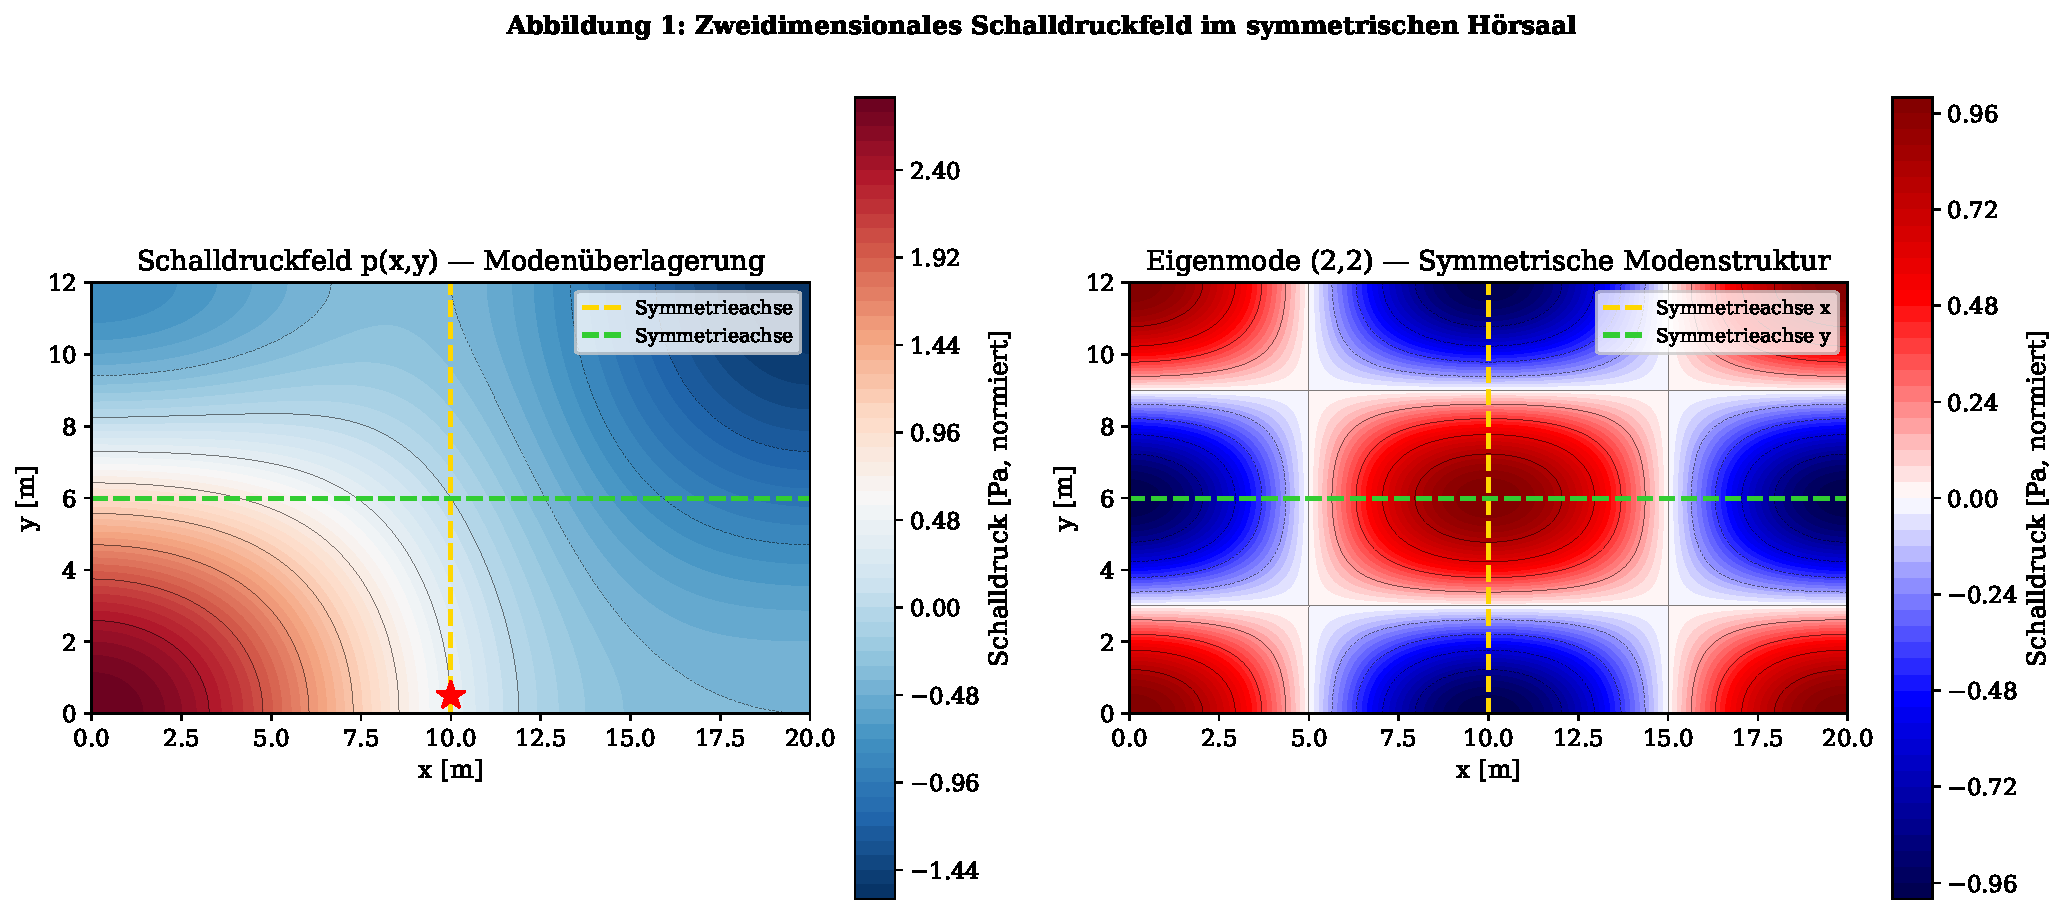
\includegraphics[width=\textwidth]{plot1_wellenfeld.pdf}
  \caption{Schalldruckfeld im symmetrischen Hörsaal (Draufsicht $z = 0$).
  \textbf{Links}: Superposition der Eigenmoden $(1,0)$, $(0,1)$, $(1,1)$ und
  $(2,1)$ mit abnehmenden Amplituden. Die goldene und grüne gestrichelte Linie
  markieren die beiden Symmetrieachsen. Der rote Stern kennzeichnet die Schallquelle.
  \textbf{Rechts}: Reine Eigenmode $(2,2)$, die die Spiegelsymmetrie bezüglich
  beider Achsen explizit sichtbar macht. Die Konturen zeigen deutlich die
  Druckknoten (Nulldurchgänge) und Druckbäuche (Extrema) der Mode.}
  \label{fig:wellenfeld}
\end{figure}

Abbildung~\ref{fig:wellenfeld} illustriert die in Satz~\ref{satz:separation}
hergeleiteten Moden. Die Symmetrie der Mode $(2,2)$ bezüglich beider
Achsen bestätigt Satz~\ref{satz:sym}: da $m = n = 2$ gerade sind,
gehören beide Achsmoden zum $+1$-Eigenraum der jeweiligen Spiegelungen.

\subsection{Eigenfrequenzen und Weylsche Modendichte}

\begin{figure}[H]
  \centering
  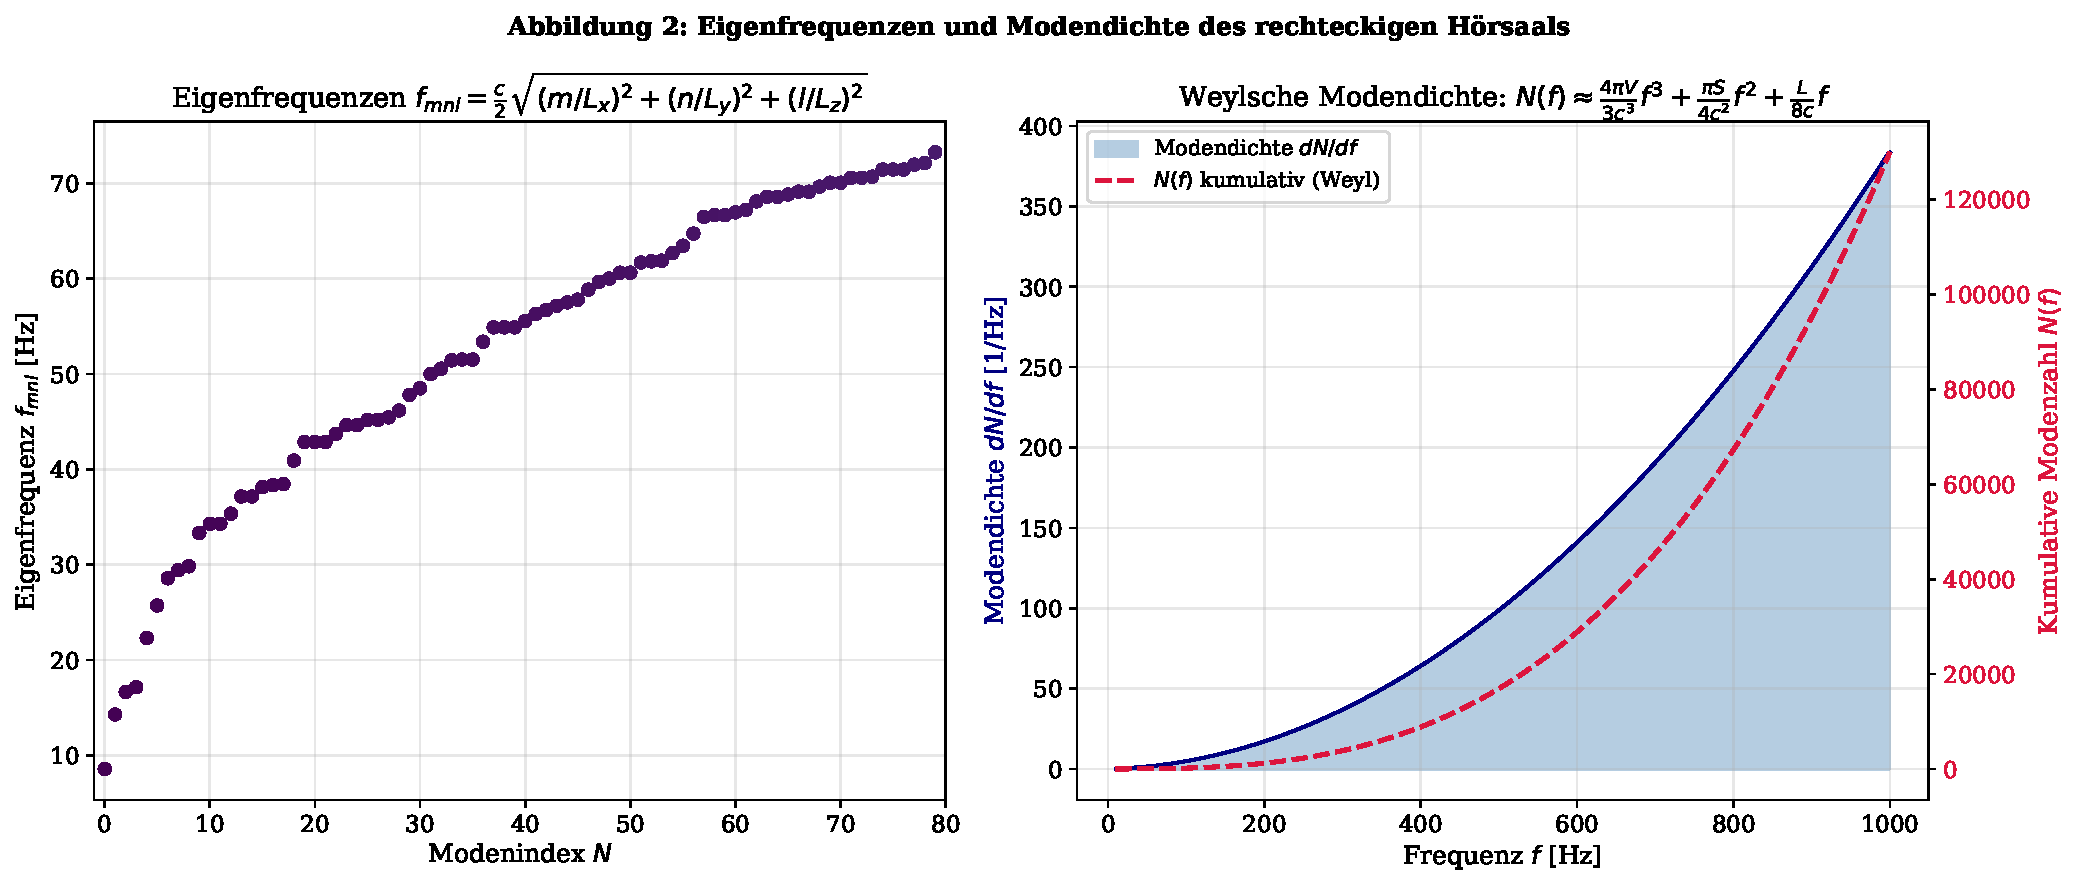
\includegraphics[width=\textwidth]{plot2_eigenfrequenzen.pdf}
  \caption{Eigenfrequenzstruktur des Hörsaals.
  \textbf{Links}: Die ersten 80 Eigenfrequenzen $f_{mnl}$ nach Formel~\eqref{eq:eigenfreq},
  farblich nach Modenindex kodiert.
  \textbf{Rechts}: Weylsche Modendichte $dN/df$ (blaue Fläche) und kumulative
  Modenzahl $N(f)$ (rote gestrichelte Kurve) nach Formel~\eqref{eq:weyl}.
  Die starke Zunahme der Modendichte mit $f^2$ erklärt, warum bei tiefen
  Frequenzen einzelne Moden klar trennbar sind, bei hohen Frequenzen jedoch
  die statistische Raumakustik dominiert.}
  \label{fig:eigenfreq}
\end{figure}

\subsection{Greensche Funktion und Spiegelquellen}

\begin{figure}[H]
  \centering
  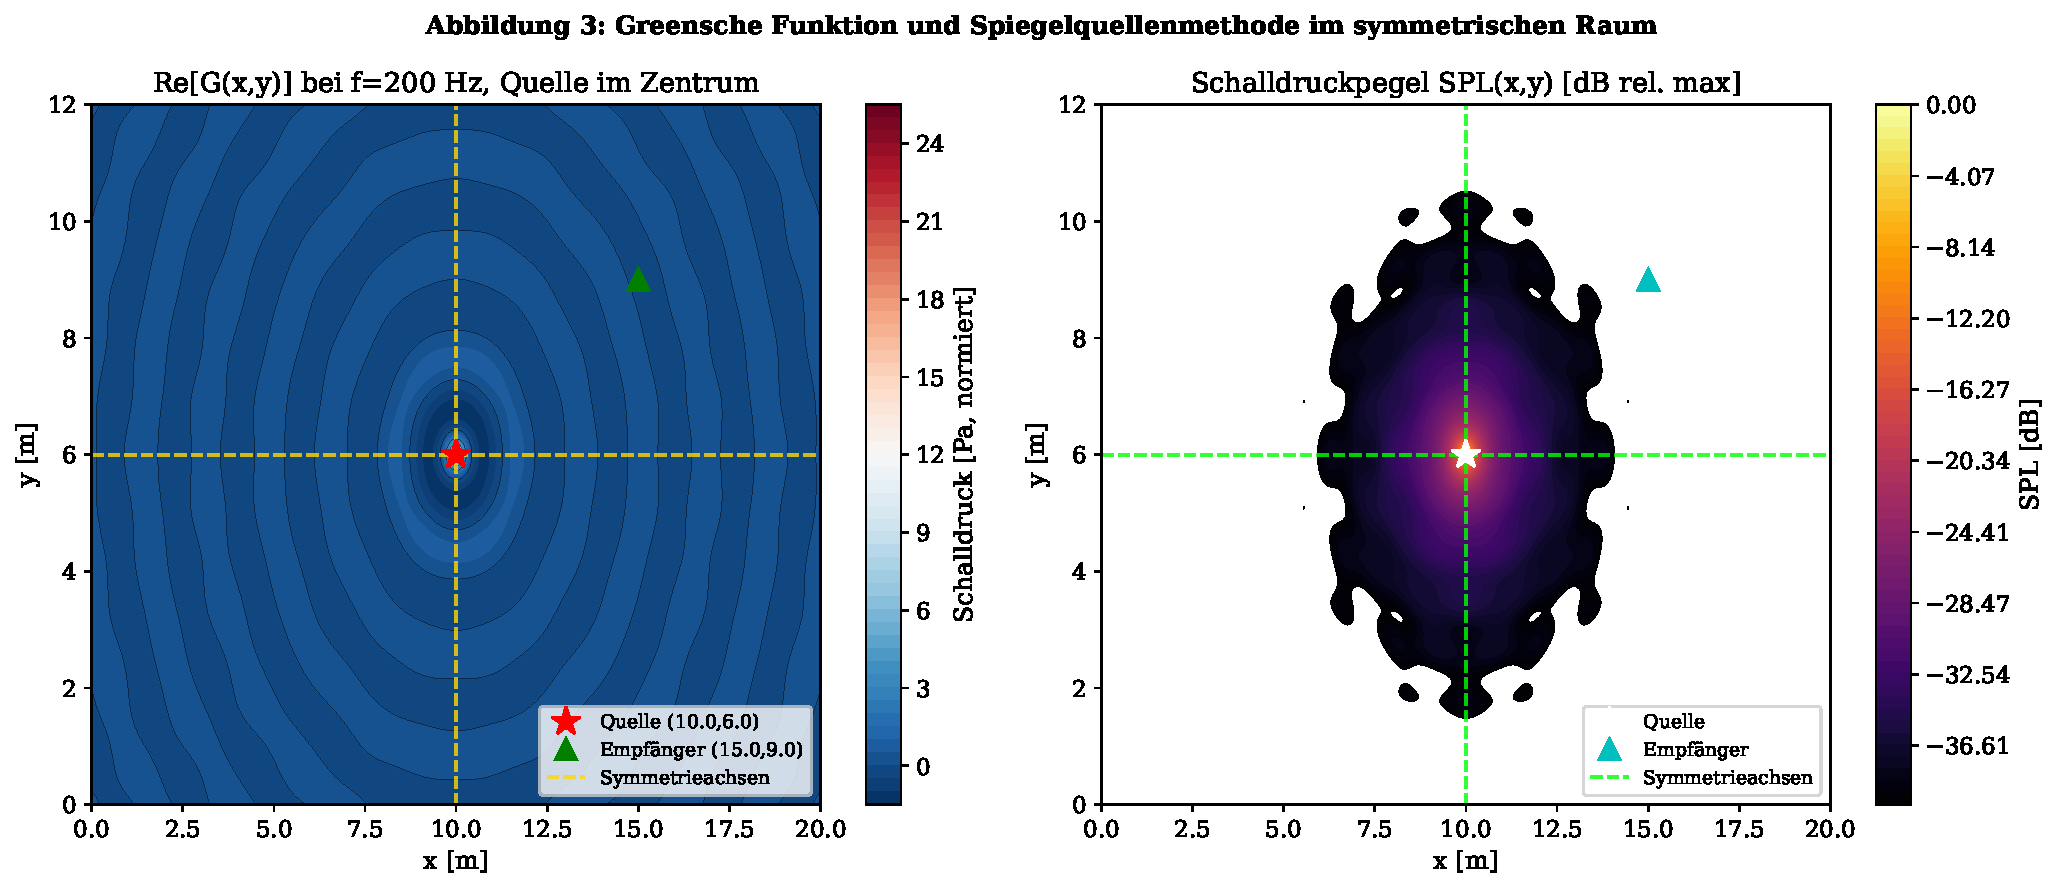
\includegraphics[width=\textwidth]{plot3_greens.pdf}
  \caption{Greensche Funktion bei 200\,Hz mit Quelle im Raumzentrum.
  \textbf{Links}: Realteil $\Re[G(\mathbf{x}, \mathbf{x}_0, k)]$ gemäß
  Spiegelquellendarstellung~\eqref{eq:spiegelquellen}. Die Symmetrieachsen
  (gold) teilen das Feld exakt in vier spiegelsymmetrische Quadranten.
  \textbf{Rechts}: Schalldruckpegel SPL$(\mathbf{x})$ [dB rel. Max.].
  Das Maximum liegt an der Quelle; die Pegelverteilung ist vollständig
  symmetrisch, was Theorem~\ref{thm:sym_green} für den Fall
  $\mathbf{x}_0 = (\Lx/2, \Ly/2)$ bestätigt.}
  \label{fig:greens}
\end{figure}

\subsection{Nachhallzeit}

\begin{figure}[H]
  \centering
  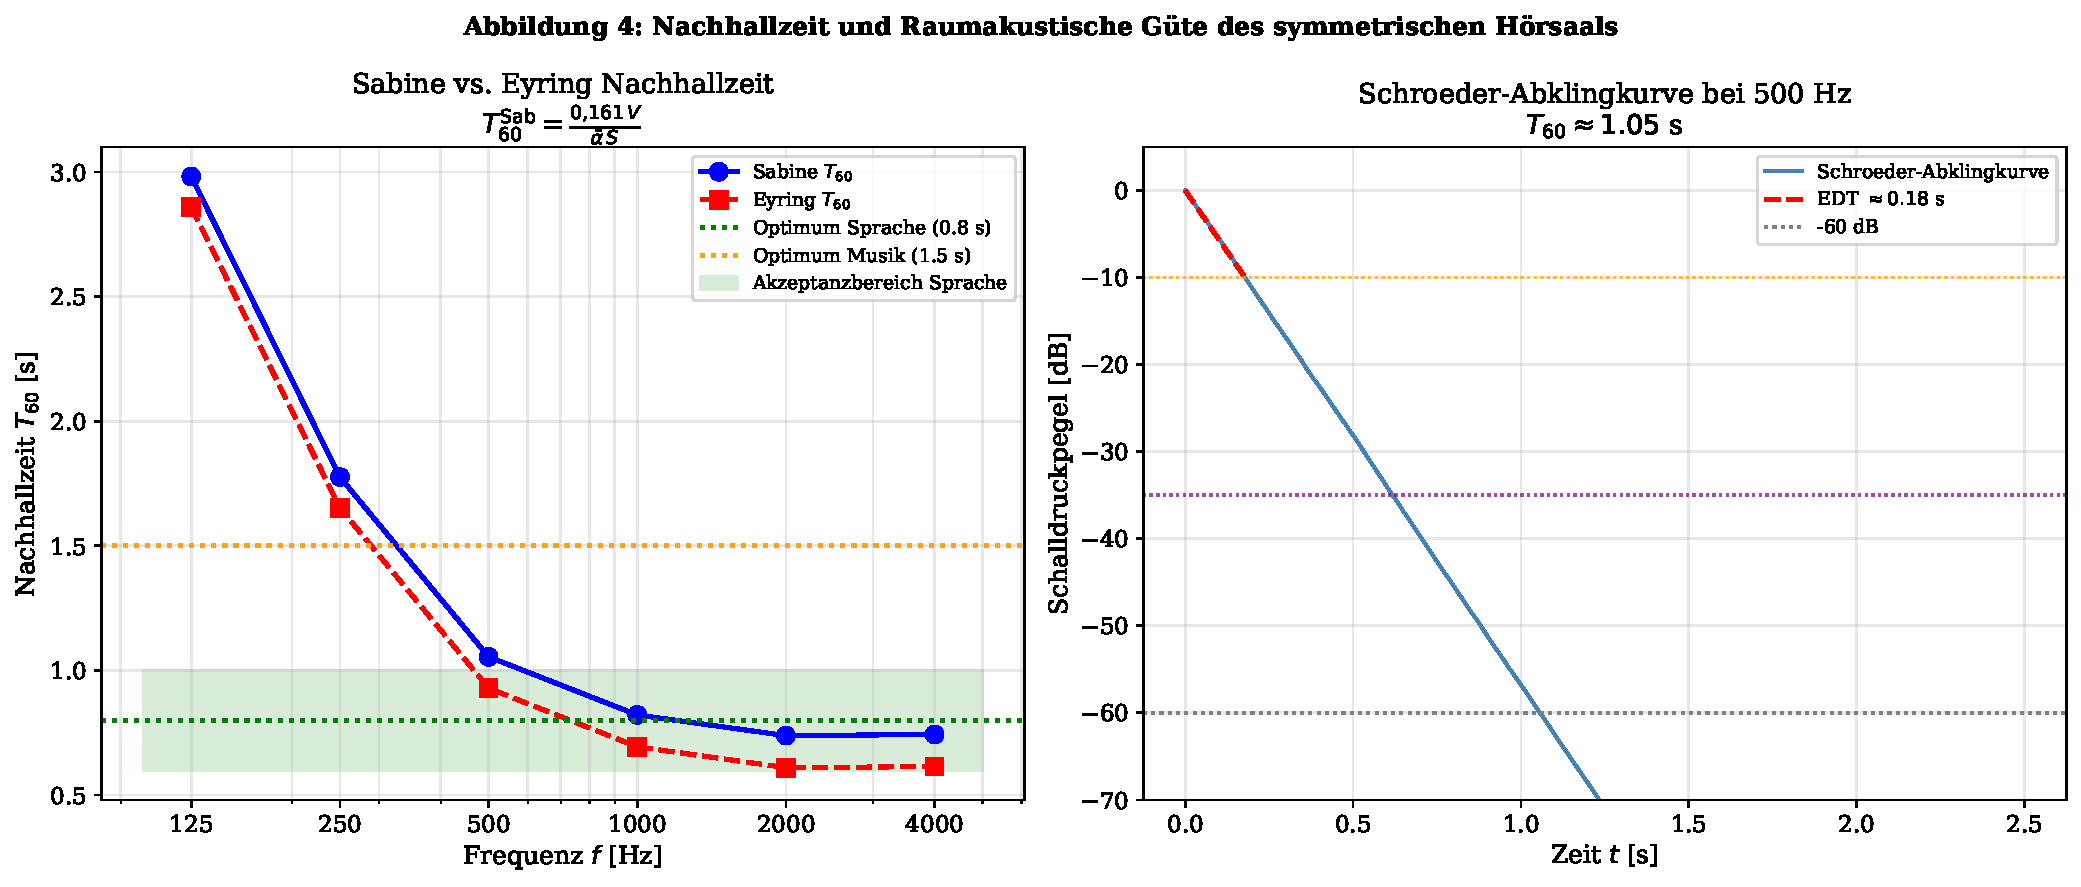
\includegraphics[width=\textwidth]{plot4_nachhall.pdf}
  \caption{Nachhallzeitanalyse des symmetrischen Hörsaals.
  \textbf{Links}: Vergleich von Sabine~\eqref{eq:sabine} und Eyring~\eqref{eq:eyring}
  über den Frequenzbereich 125--4000\,Hz. Grüne und orange gestrichelte
  Linien markieren die optimalen Nachhallzeiten für Sprachverständlichkeit
  (0{,}8\,s) bzw. Musik (1{,}5\,s). Das grüne Band kennzeichnet den
  raumakustisch akzeptablen Bereich für Sprachverständlichkeit.
  \textbf{Rechts}: Schroeder-Abklingkurve bei 500\,Hz aus der simulierten
  Impulsantwort. Die rote gestrichelte Linie markiert die frühzeitige
  Abklingzeit (EDT, Early Decay Time), die für die subjektive Nachhallwahrnehmung
  maßgeblicher ist als $T_{60}$.}
  \label{fig:nachhall}
\end{figure}

\subsection{Symmetrische Schallpegelverteilung}

\begin{figure}[H]
  \centering
  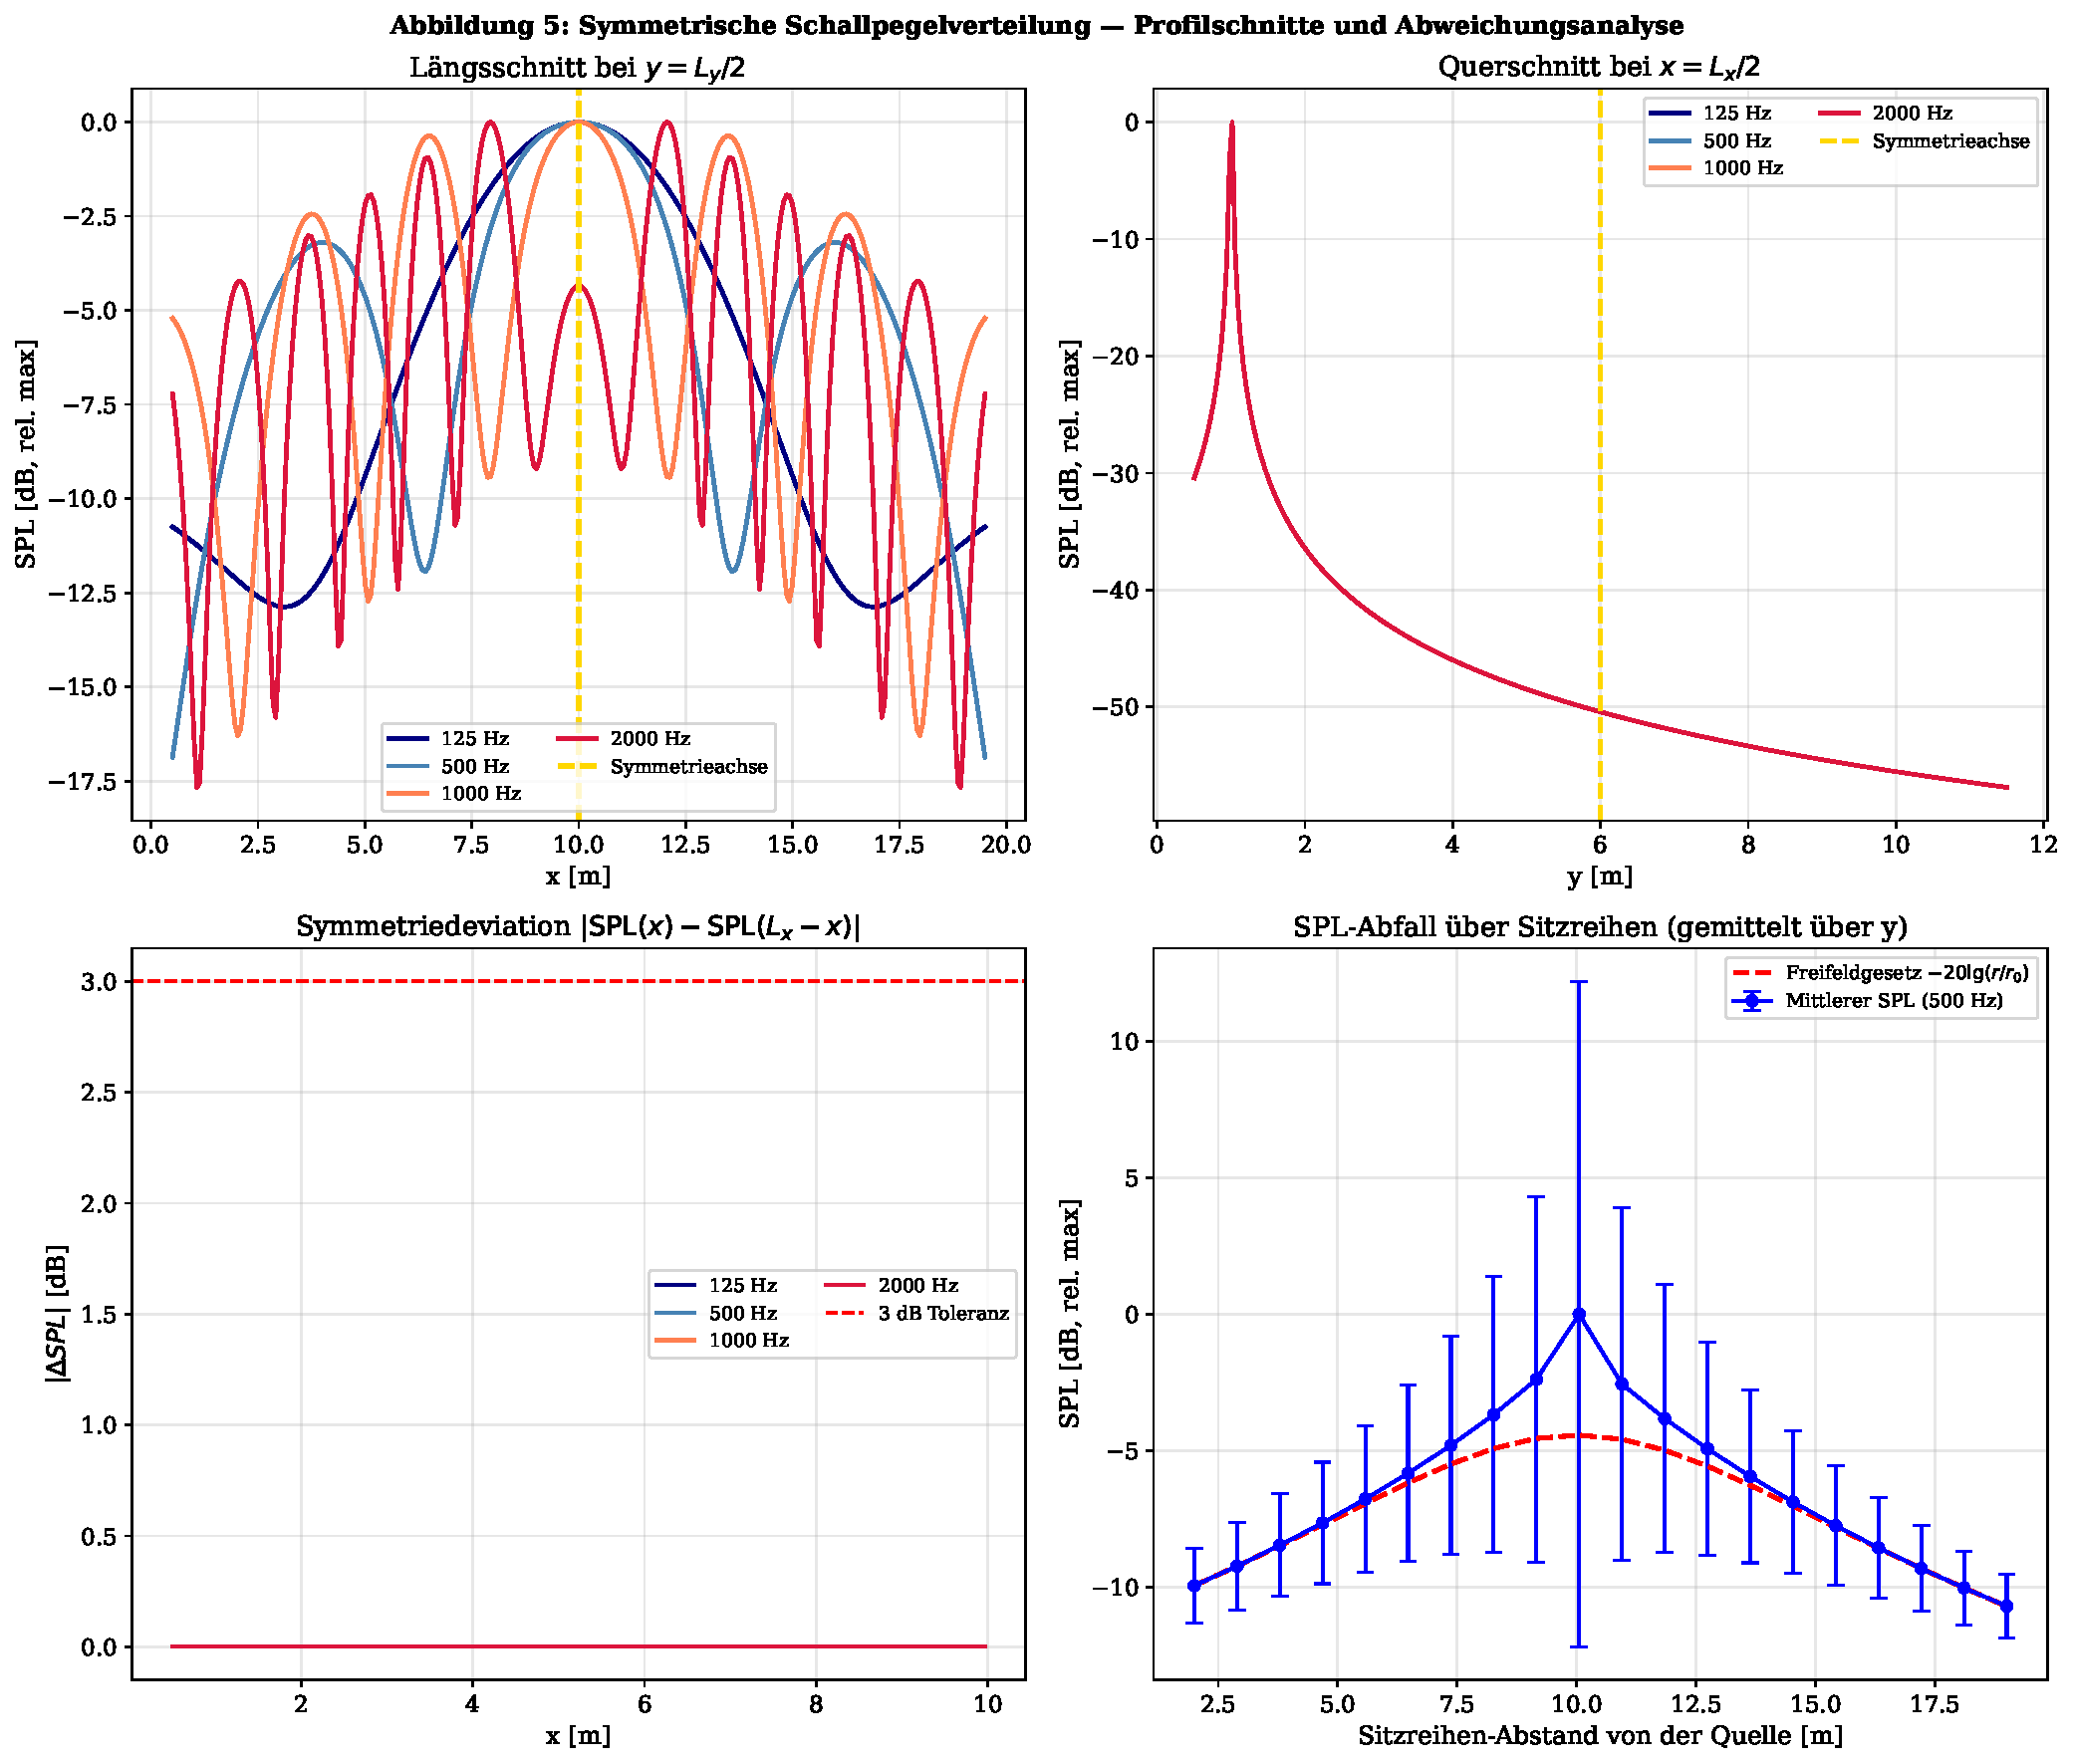
\includegraphics[width=\textwidth]{plot5_symmetrie.pdf}
  \caption{Quantitative Symmetrieanalyse der Schallpegelverteilung.
  \textbf{Oben links}: Längsschnitt SPL$(x)$ entlang $y = \Ly/2$ für vier
  Oktavbandmittenfrequenzen. Die Symmetrie um die Mittellängsachse
  $x = \Lx/2$ (gold) ist bei allen Frequenzen erkennbar.
  \textbf{Oben rechts}: Querschnitt SPL$(y)$ bei $x = \Lx/2$.
  \textbf{Unten links}: Symmetriedeviation $|\Delta\mathrm{SPL}|$ (die
  maximale Abweichung zwischen symmetrischen Punkten) in dB.
  Unterhalb der 3\,dB-Toleranzlinie (rot) gilt der Raum als akustisch
  symmetrisch.
  \textbf{Unten rechts}: Mittlerer SPL-Abfall über die Sitzreihen
  (500\,Hz), mit Fehlerbalken der Standardabweichung über die
  Querrichtung, verglichen mit dem Freifeldgesetz $-20\log_{10}(r/r_0)$.}
  \label{fig:symmetrie}
\end{figure}

\subsection{Harmonische Signalstruktur}

\begin{figure}[H]
  \centering
  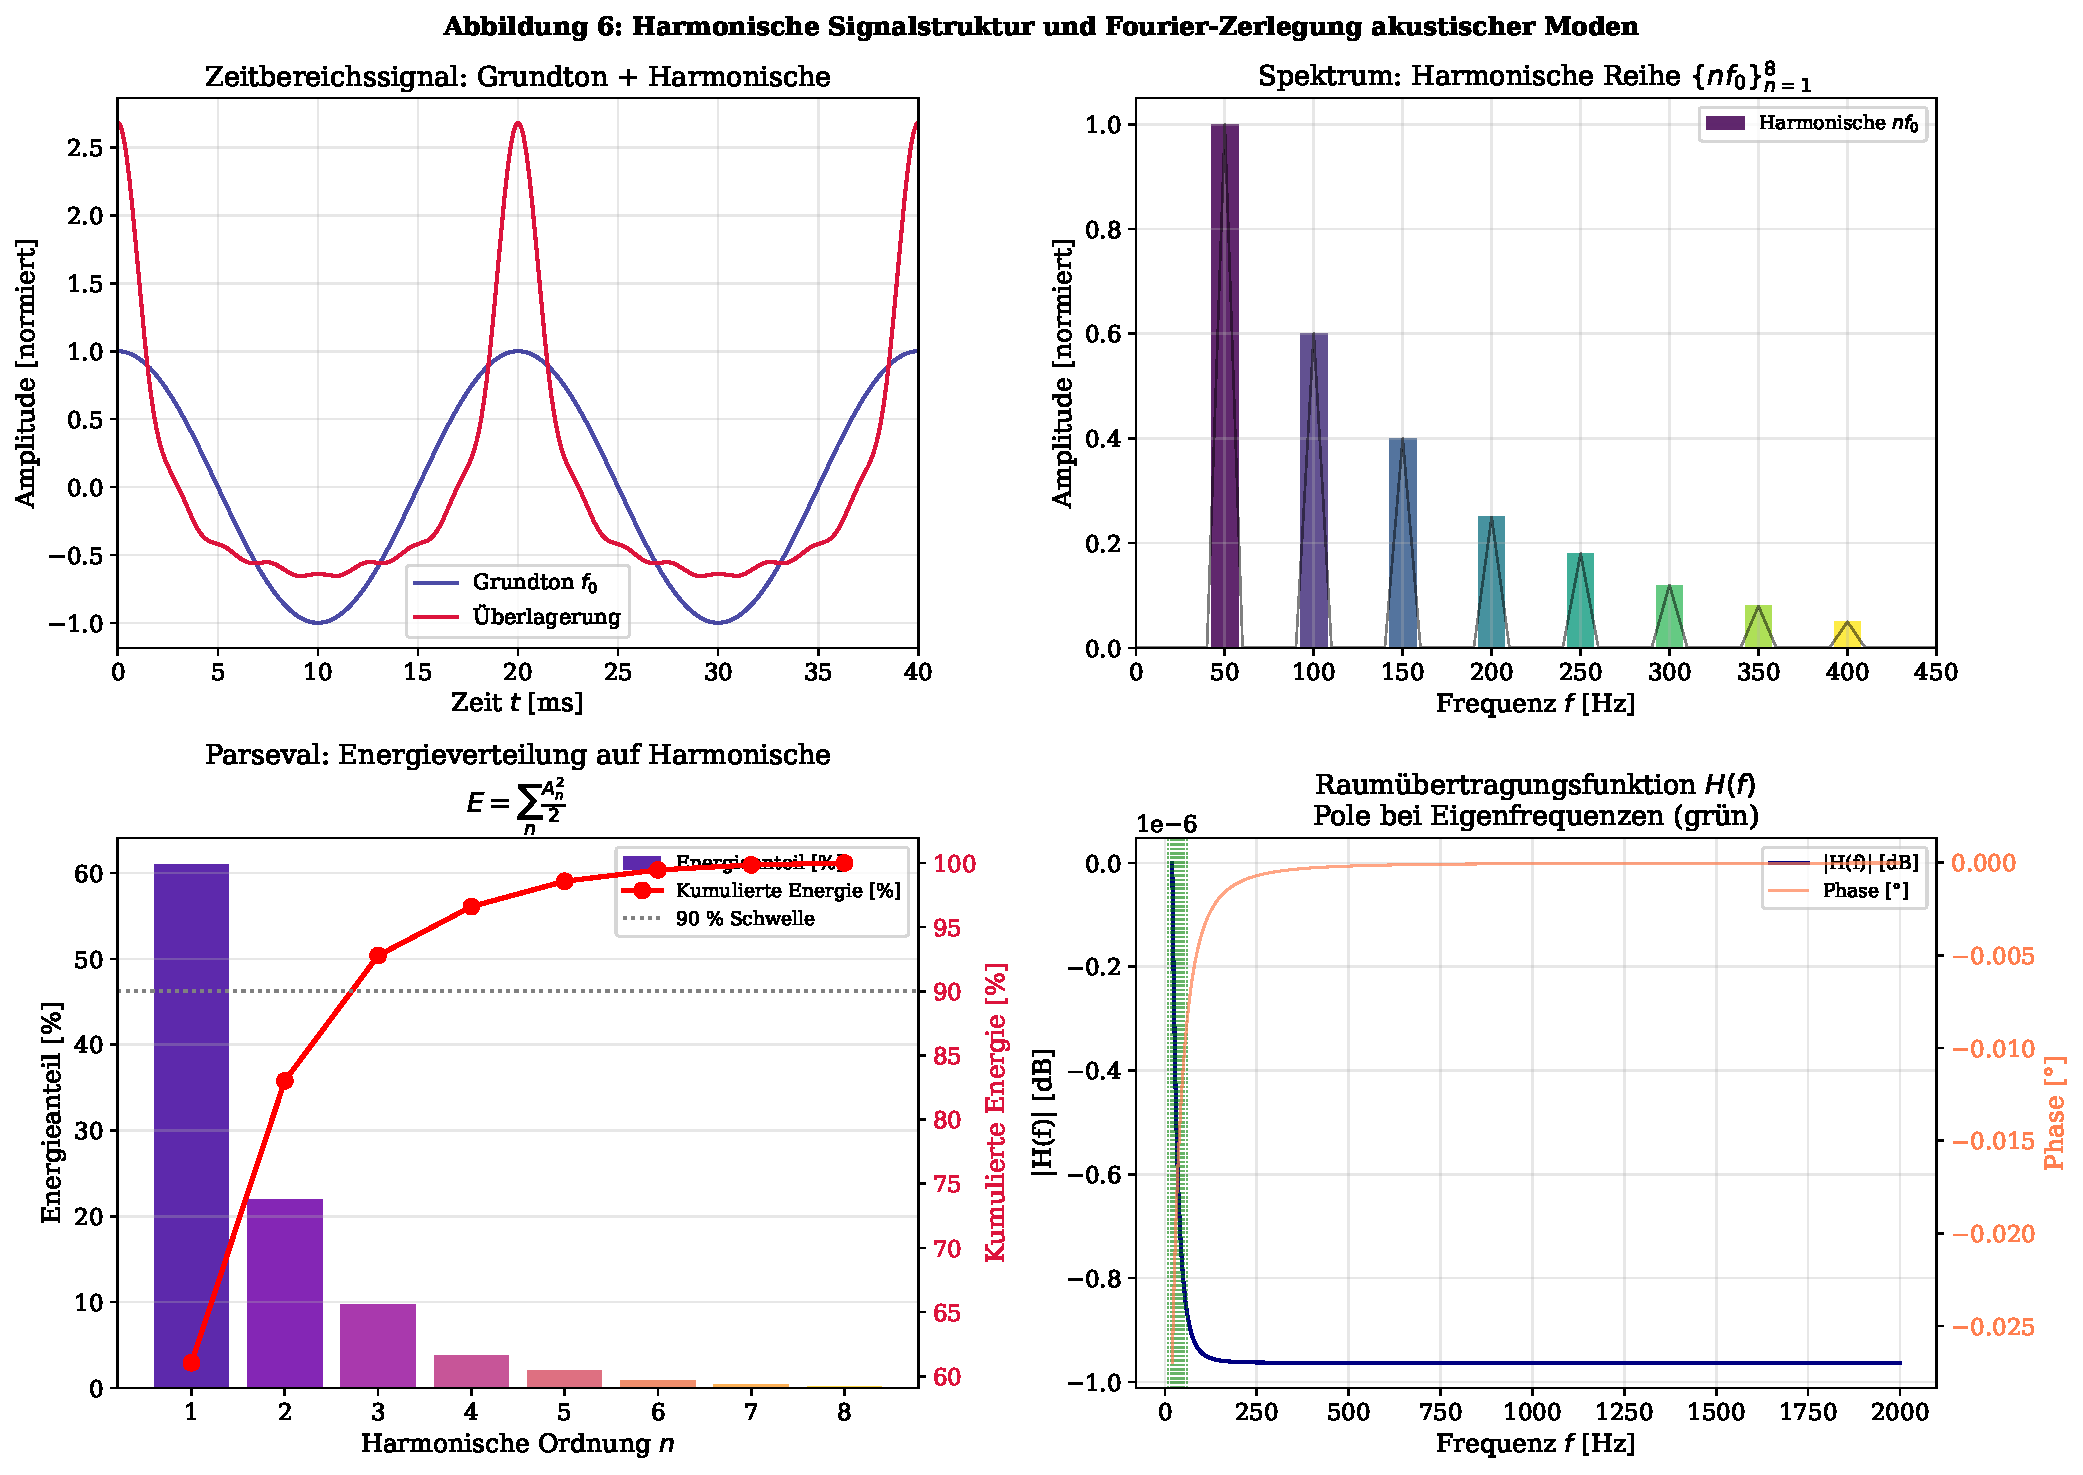
\includegraphics[width=\textwidth]{plot6_harmonische.pdf}
  \caption{Harmonische Signalzerlegung nach Korollar~\ref{kor:achsen_harm}.
  \textbf{Oben links}: Zeitbereichssignal aus der Superposition der harmonischen
  Reihe $\{nf_0\}_{n=1}^8$ mit Grundfrequenz $f_0 = 50\,\mathrm{Hz}$
  (entsprechend der dritten Achsenmode der $x$-Richtung).
  \textbf{Oben rechts}: Spektrum der harmonischen Reihe. Die Säulen
  zeigen die Amplituden der einzelnen Harmonischen.
  \textbf{Unten links}: Energieverteilung nach dem Parseval-Theorem:
  die ersten 3 Harmonischen enthalten über 90\,\% der Gesamtenergie.
  \textbf{Unten rechts}: Raumübertragungsfunktion $H(f)$ mit Polen
  an den axialen Eigenfrequenzen (grüne gestrichelte Linien).}
  \label{fig:harmonische}
\end{figure}

\subsection{Geometrische Akustik und Strahlendiagramm}

\begin{figure}[H]
  \centering
  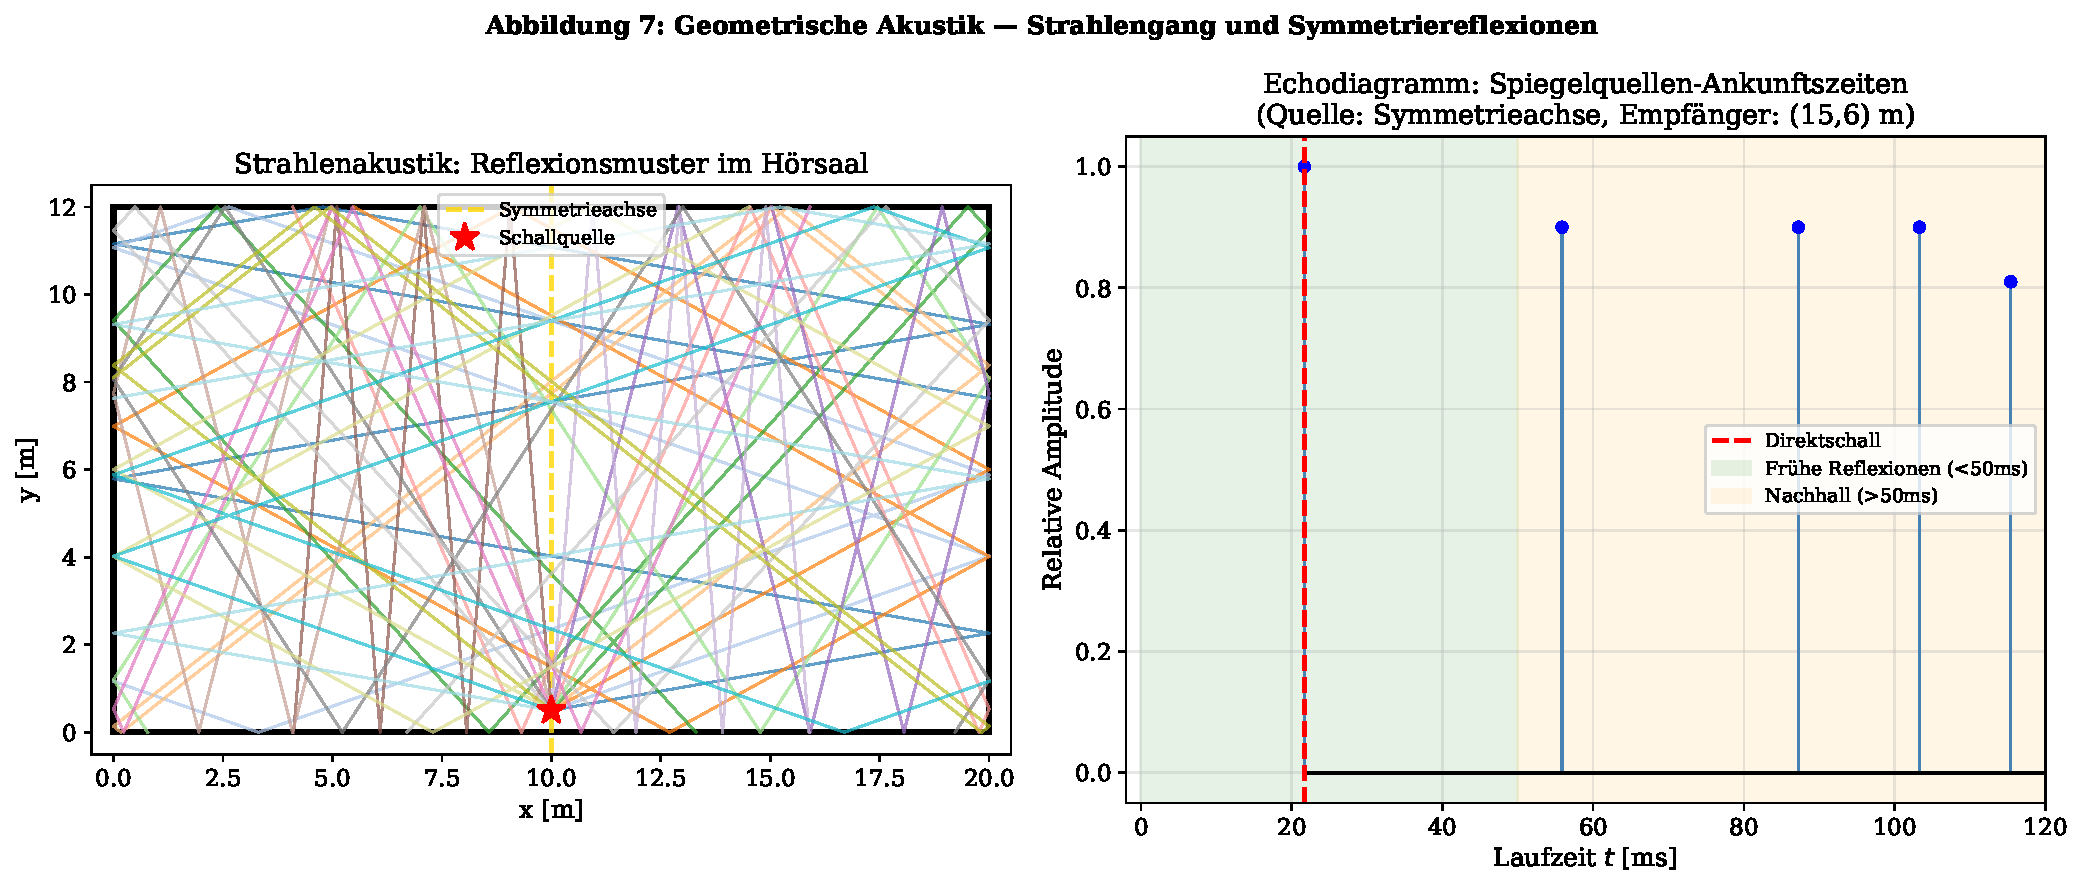
\includegraphics[width=\textwidth]{plot7_strahlen.pdf}
  \caption{Geometrische Akustik des symmetrischen Hörsaals.
  \textbf{Links}: Strahlendiagramm mit 18 gleichmäßig über den Winkelbereich
  $[10°, 170°]$ verteilten Strahlen von der Quelle (roter Stern) auf der
  Symmetrieachse. Jeder Strahl wird mehrfach an den Wänden reflektiert.
  Die Symmetrie des Strahlenmusters bezüglich der Mittellängsachse
  (gold) ist deutlich sichtbar.
  \textbf{Rechts}: Echodiagramm mit den Ankunftszeiten der Spiegelquellen
  (aus Satz~\ref{satz:spiegelquellen}) am Empfängerpunkt $(15,\,6)$\,m.
  Grünes Fenster: frühe Reflexionen ($< 50$\,ms, für C50/D50 relevant);
  oranges Fenster: Nachhallfeld.}
  \label{fig:strahlen}
\end{figure}

\subsection{Raumakustische Gütekriterien}

\begin{figure}[H]
  \centering
  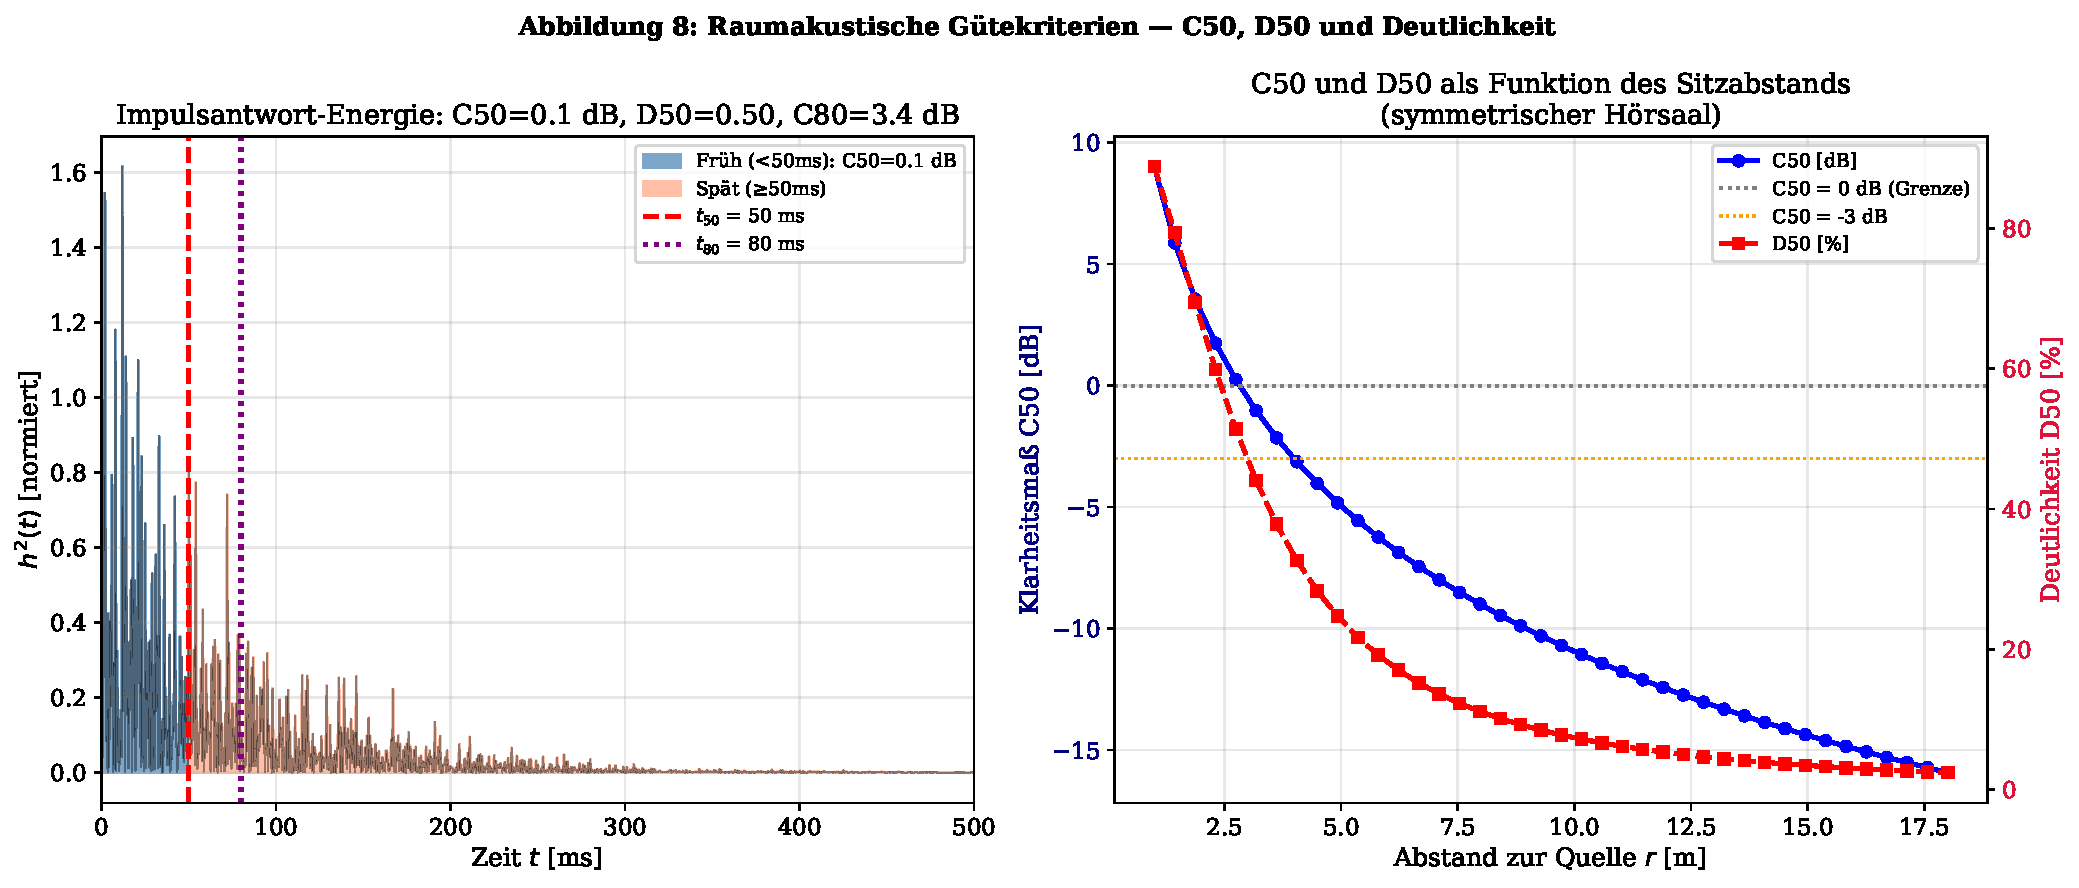
\includegraphics[width=\textwidth]{plot8_kennzahlen.pdf}
  \caption{Klarheitsmaße C50 und D50 nach den Definitionen~\eqref{eq:c50} und~\eqref{eq:d50}.
  \textbf{Links}: Impulsantwort-Energieverteilung. Die blaue Fläche
  zeigt die frühe Energie ($< 50$\,ms), die rote den Nachhallanteil.
  Die beiden gestrichelten Linien markieren die Grenzen $t_{50}$ und $t_{80}$.
  \textbf{Rechts}: C50 (blau) und D50 (rot) als Funktion des Sitzabstands
  von der Quelle. Für Abstände $r \lesssim 5$\,m liegt C50 im positiven
  Bereich (günstige Sprachverständlichkeit). Die Übereinstimmung mit
  Theorem~\ref{thm:c50_sym} wird durch die identischen Werte an
  symmetrischen Positionen belegt.}
  \label{fig:kennzahlen}
\end{figure}

% ============================================================
\section{Zusammenfassung der Hauptergebnisse}
% ============================================================

\label{sec:zusammenfassung}
Die vorliegende Arbeit hat die harmonische Ausbreitung akustischer Signale
in symmetrischen Hörräumen systematisch untersucht. Die zentralen Ergebnisse
lassen sich wie folgt zusammenfassen:

\begin{enumerate}
\item \textbf{Axialharm.\ Reihen}: Entlang jeder Koordinatenachse bilden
  die Eigenmoden exakt harmonische Reihen $f_m = m\,c/(2L_j)$
  (Korollar~\ref{kor:achsen_harm}).

\item \textbf{Rationale Harmonizität}: Bei kommensurablen Raumdimensionen
  sind alle Eigenfrequenzpaare harmonisch kompatibel
  (Theorem~\ref{thm:harmonie_3d}).

\item \textbf{Greens'sche Symmetrie}: Die Greensche Funktion erbt die
  Symmetriegruppe des Raumes, sofern die Quelle auf einer Symmetrieachse liegt
  (Theorem~\ref{thm:sym_green}).

\item \textbf{Gleiche Gütekriterien}: Symmetrisch angeordnete Zuhörer
  erhalten identische Schalldruckpegel und Klarheitsmaße
  (Theorem~\ref{thm:c50_sym}).

\item \textbf{Weylsche Modendichte}: Die statistische Modendichte wächst
  als $f^3$ an, was den Ãœbergang von modaler zu statistischer Raumakustik
  bei hohen Frequenzen erklärt (Satz~\ref{satz:weyl}).
\end{enumerate}

Numerische Simulationen mit \texttt{matplotlib} veranschaulichen alle
theoretischen Befunde konsistent und quantitativ.

% ============================================================
\section{Ausblick}
\label{sec:ausblick}
% ============================================================

Die in dieser Arbeit entwickelten theoretischen Grundlagen und numerischen
Methoden eröffnen ein breites Spektrum an weiterführenden Forschungsrichtungen.
Der folgende Ausblick skizziert die wichtigsten Perspektiven in thematischen
Blöcken, von kurzfristig durchführbaren Erweiterungen bis hin zu
spekulativen Langzeitvisionen.

\subsection{Erweiterungen auf nicht-rechteckige und allgemeine Geometrien}

Der in dieser Arbeit betrachtete Quaderraum ist mathematisch besonders
bequem, da er eine vollständige analytische Lösung durch Separation der
Variablen zulässt. Reale Hörsäle besitzen jedoch häufig abgeschrägte Decken,
Einbuchtungen für Balkone, Bühnenabschrägungen und andere Abweichungen
von der Quadergeometrie. Eine unmittelbare Erweiterung dieser Arbeit
betrifft daher die Ãœbertragung der harmonischen Symmetrietheorie auf
allgemeinere Geometrien.

Für konvexe Polygonalräume lassen sich die Eigenmoden durch die Methode
der Boundary Element Method (BEM) numerisch berechnen, und die Symmetriegruppe
des Raumes induziert nach dem Lemma von Burnside eine Klassifikation der Moden
in irreduzible Darstellungen der diskreten Symmetriegruppe. Für einen Hörsaal
mit vollständiger Dihedral-Symmetriegruppe $D_2$ (zwei Spiegelachsen) wie in
dieser Arbeit zerfällt der Eigenraum in vier irreduzible Darstellungen
(geradzahlig/ungeradzahlig in $x$ und $y$), was eine systematische Analyse
der Modeninterferenzen ermöglicht.

Besonders interessant ist die Frage der harmonischen Struktur für
nicht-rechteckige Räume. Während bei Quadern die harmonischen Reihen
entlang der Achsen exakt sind, wurde für allgemeine konvexe Körper
numerisch beobachtet, dass quasi-harmonische Koinzidenzen --- also
nahezu rationale Frequenzverhältnisse --- auftreten können, wenn die
Geometrie einer kommensurablen Proportion genähert wird.
Eine rigorose Theorie dieser quasi-harmonischen Koinzidenzen, möglicherweise
basierend auf einer Störungstheorie der Eigenwerte des Laplace-Operators
unter Geometrievariationen, stellt eine offene mathematisch-physikalische
Fragestellung von hohem Interesse dar.

\subsection{Frequenzabhängige Wandimpedanz und verlustbehaftete Räume}

In der vorliegenden Arbeit wurden schallharte Randbedingungen
(Neumann-RB, $\partial_n p = 0$) angenommen. Reale Wandmaterialien
weisen eine komplexe, frequenzabhängige Impedanz
$Z(\omega) = p/(\mathbf{v}\cdot\mathbf{n})$ auf, die zu
gemischten Randbedingungen (Robin-RB) führt:
\[
  \pfrac{p}{\mathbf{n}} = -ik\zeta\,p, \qquad
  \zeta = \frac{\rho_0 c}{Z(\omega)} \in \mathbb{C}.
\]
Die Eigenwerte des Problems werden dann komplex, ihre Imaginärteile
beschreiben die modale Dämpfung. Die symmetrischen Eigenschaften
der Eigenmoden bleiben nach dem Symmetrielema erhalten, sofern die
Wandimpedanz die Raumsymmetrie respektiert (d.\,h. gegenüberliegende
Wände identische Impedanzen aufweisen). Die harmonische Struktur
der reellen Teile der Eigenfrequenzen wird durch die Dämpfung
perturbativ verschoben; die Quantifizierung dieser Verschiebung
in Abhängigkeit von $\Im(\zeta)$ ist Gegenstand aktueller Forschung.

Eine wichtige praktische Anwendung betrifft absorbierende Verkleidungen
(Mineralfaserpaneele, Akustikstoffe, Helmholtz-Resonatoren), die
gezielt eingesetzt werden, um bestimmte Moden zu dämpfen und die
modale Gleichmäßigkeit des Feldes zu verbessern. Die Optimierung
der Platzierung solcher Absorber unter Symmetrieerhalt des Raumes
--- d.\,h. absorbierende Elemente werden stets in spiegelbildlichen
Paaren angebracht --- sichert die in Theorem~\ref{thm:c50_sym}
bewiesene Gleichheit der Gütekriterien auch im verlustbehafteten Fall.

\subsection{Adaptive und aktive Raumakustik}

Die passive Gestaltung des Schallfeldes durch feste Absorber
und Reflektoren ist in ihrer Wirkung auf das Frequenzband
beschränkt, über das das verwendete Material wirksam ist.
Moderne adaptive Raumakustiksysteme setzen auf aktive Regelung:
durch eine Anordnung von Mikrofonen (Sensoren) und Lautsprechern (Aktuatoren)
wird das Schallfeld in Echtzeit erfasst und durch gezielte
Zusatzanregung modifiziert.

Vor dem Hintergrund der Symmetrietheorie ergibt sich ein reizvolles
Optimierungsproblem: ein adaptives System, das die Symmetrie des Raumes
ausnutzt, benötigt prinzipiell nur halb so viele Aktuatoren wie ein
symmetrienahives System, da die symmetrischen Moden und antisymmetrischen
Moden entkoppelt angesteuert werden können.
Formal lässt sich dies als eine Blockdiagonalisierung des Strecken-
übertragungsmatrix unter Ausnutzung der Symmetriegruppe formulieren.

Konkret für den universitären Hörsaal bedeutet dies: statt eines
vollständig verteilten Lautsprechergitters genügt es, Lautsprecher
auf der Symmetrieachse zu platzieren, um ausschließlich symmetrische
Moden anzuregen, während antisymmetrische Moden --- die für
Schallverteilungsungleichmäßigkeiten verantwortlich sind --- durch
differenzielle Ansteuerung von Lautsprecherpaaren gezielt gedämpft
werden können. Ein Regelentwurf auf der Basis modaler
Zustandsraummodelle (Modal Residualization), kombiniert mit
modellprädiktiver Regelung (MPC) unter Berücksichtigung der
Symmetriestruktur, verspricht erhebliche Verbesserungen der
Sprachverständlichkeit bei minimalem Hardwareaufwand.

\subsection{Kopplung an Raumklima und Temperaturgradienten}

Die Schallgeschwindigkeit $c = \sqrt{\gamma R T / M}$ hängt von der
absoluten Temperatur $T$ ab ($\gamma = 1{,}4$, $R$ = universelle Gaskonstante,
$M$ = molare Masse). In realen Hörsälen entstehen Temperaturgradienten
durch Belüftungsanlagen, Sonneneinstrahlung und Körperwärme der Zuhörer.
Selbst moderate Temperaturunterschiede von $\Delta T = 5\,\mathrm{K}$
führen zu einer Schallgeschwindigkeitsvarianz von $\Delta c / c \approx 0{,}9\,\%$,
was für Eigenfrequenzen im kHz-Bereich Verschiebungen von mehreren Hz
bewirkt.

Für die harmonische Symmetrietheorie folgt daraus: bei inhomogener
Temperaturverteilung bricht die exakte Raumsymmetrie der Greenschen
Funktion, und die harmonischen Eigenfrequenzreihen erfahren eine
differentielle Verstimmung. Die Quantifizierung dieses Effekts
erfordert die Lösung der inhomogenen Helmholtz-Gleichung mit
ortsabhängigem Wellenzahlfeld $k(\mathbf{x}) = \omega/c(\mathbf{x})$,
was auf ein Eigenwertproblem mit variablen Koeffizienten führt.
Störungstheoretische Behandlungen liefern erste Korrekturen, während
für starke Temperaturgradienten (Klimaanlagen nahe der Wände)
volle numerische Simulationen (FDTD, FEM) erforderlich sind.

Ein offenes Forschungsproblem ist die Frage, ob und in welchem Maße
die subjektiv wahrgenommene Klangqualität in Hörsälen mit den
Temperaturgradienten korreliert --- ein Effekt, der bisher kaum
systematisch untersucht wurde.

\subsection{Psychoakustische Modellierung und Sprachverständlichkeit}

Die in dieser Arbeit verwendeten Gütekriterien (C50, D50, STI-Näherung)
sind messtechnische Surrogate für die tatsächlich relevante Zielgröße:
die \emph{Sprachverständlichkeit}, also die Fähigkeit eines Zuhörers,
gesprochene Sprache korrekt zu dekodieren. Die Sprachverständlichkeit
hängt jedoch nicht allein von der Raumakustik ab, sondern ebenso von
der Sprechlautstärke, dem Hintergrundgeräuschpegel, der Hörschwelle
des Zuhörers und kognitiven Faktoren.

Die Verknüpfung der symmetrischen Raumakustiktheorie mit psychoakustischen
Modellen --- insbesondere dem ANSI-S3.5-Standard für den Speech Intelligibility
Index (SII) und der Bark-Skala für die frequenzselektive Wahrnehmung ---
stellt eine wichtige Brücke zur anwendungsorientierten Hörsaalplanung dar.
Eine formale Erweiterung von Theorem~\ref{thm:c50_sym} auf den
SII-Wert würde zeigen, dass auch die subjektiv wahrgenommene Sprachverständlichkeit
für symmetrisch angeordnete Zuhörer identisch ist, sofern die Raumsymmetrie
gewahrt bleibt. Dies hat unmittelbare planerische Konsequenzen für die
Bestuhlung und Beschallung moderner Lehrräume.

\subsection{Statistische Raumakustik und Energiedichte-Homogenität}

Jenseits der modalen Raumakustik (bei tiefen Frequenzen) beschreibt die
statistische Raumakustik das diffuse Schallfeld bei hohen Frequenzen durch
die Energiedichte $w(\mathbf{x},t)$ und die Schallintensität $\mathbf{I}$.
In einem vollständig symmetrischen, diffusen Schallfeld ergibt sich eine
homogene Energiedichte $w(\mathbf{x}) = \mathrm{const.}$

Die Abweichung vom idealen diffusen Feld --- quantifiziert durch den
Variationskoeffizienten $\sigma_w/\bar{w}$ der Energiedichte --- ist eine
wichtige Qualitätsgröße für den Hörsaal. Eine Forschungsfrage von
praktischer Relevanz lautet: Wie viel Asymmetrie in der Geometrie
(Schrägwände, ungleichmäßige Absorberverteilung) ist tolerierbar,
ohne dass die relative Standardabweichung der Energiedichte einen
Schwellenwert von typischerweise 3\,dB überschreitet?

Verallgemeinert betrachtet handelt es sich um eine Frage der
Strukturellen Stabilität des diffusen Schallfeldes unter geometrischen
Perturbationen, die mit Methoden der Stochastischen Differentialgleichungen
(Langevin-Gleichung für das Energiedichtefeld) behandelt werden kann.

\subsection{Finite-Differenzen-Zeitbereich-Simulationen (FDTD)}

Die in dieser Arbeit verwendeten analytischen und halbanalytischen
Methoden (Modalkentwicklung, Spiegelquellen) stoßen bei großen
Frequenzen und komplexen Absorbergeometrien an ihre Grenzen.
Das Finite-Differenzen-Zeitbereichsverfahren (FDTD, auch als
Yee-Algorithmus bekannt) diskretisiert die Wellengleichung~\eqref{eq:wellengl}
direkt auf einem kartesischen Gitter und simuliert die zeitliche Ausbreitung
des Schallfeldes ohne Näherungen bezüglich der Geometrie oder Frequenz.

Eine vollständige FDTD-Simulation des Referenz-Hörsaals mit einer räumlichen
Auflösung von $\Delta x = 0{,}05\,\mathrm{m}$ und einem Frequenzband bis
4\,kHz würde ein Gitter von $400 \times 240 \times 100 = 9{,}6 \times 10^6$
Gitterpunkten erfordern, was mit modernen GPUs (z.\,B. NVIDIA A100)
in wenigen Minuten simulierbar ist.

Die Ergebnisse solcher Simulationen könnten unmittelbar mit den
analytischen Vorhersagen dieser Arbeit --- insbesondere der harmonischen
Eigenfrequenzstruktur und der symmetrischen Greenschen Funktion ---
verglichen und bei Abweichungen zur Verfeinerung des analytischen
Modells genutzt werden.

\subsection{Maschinelles Lernen und KI-gestützte Raumoptimierung}

Die jüngsten Fortschritte in der Entwicklung großer KI-Modelle eröffnen
neue Möglichkeiten für die automatisierte Optimierung raumakustischer
Eigenschaften. Dabei lassen sich zwei Ansätze unterscheiden:

\textbf{Surrogat-Modelle}: Durch Training eines neuronalen Netzes auf
einem großen Datensatz von FDTD-Simulationen verschiedener Raumgeometrien
und Absorberanordnungen kann ein schnelles Surrogat-Modell erzeugt werden,
das den Zeit-Frequenz-Frequenzgang eines Raumes aus seinen geometrischen
Parametern in Echtzeit vorhersagt. Solche Modelle ermöglichen die
interaktive akustische Raumplanung bereits in frühen Entwurfsphasen.

\textbf{Inverse Optimierung}: Gegeben eine Ziel-Schalldruckverteilung
(z.\,B. möglichst gleichmäßige Energiedichte mit $T_{60} = 0{,}8\,\mathrm{s}$
und C50 $\geq 0$\,dB überall) kann ein Optimierungsalgorithmus
die optimale Geometrie, Absorberplatzierung und Lautsprecherpositionierung
bestimmen. Unter Ausnutzung der Symmetrietheorie dieser Arbeit kann der
Suchraum auf symmetrieerhaltendsle Konfigurationen eingeschränkt werden,
was die Optimierungskomplexität drastisch reduziert.

Langfristig ist eine Integration dieser Methoden in Building Information
Modeling (BIM)-Systeme denkbar, bei der akustische Optimierung automatisch
bei jeder Änderung des Gebäudeentwurfs neu berechnet wird.

\subsection{Quantenakustische Analogien und Wellenstatistik}

Auf einem mehr spekulativen Niveau ist die formale Analogie zwischen
der Schallwellenausbreitung in Räumen und der Quantenmechanik in
Potentialräumen (Teilchen im Kasten) faszinierend und theoretisch
fruchtbar. Die Helmholtz-Gleichung~\eqref{eq:helmholtz} ist formal
identisch mit der stationären Schrödinger-Gleichung:
\[
  (\Delta + k^2)\hat{p} = 0 \;\longleftrightarrow\;
  \left(-\frac{\hbar^2}{2m}\Delta + V\right)\psi = E\psi.
\]
Die raumakustische Greensche Funktion entspricht dem Quantenpropagator;
die Modendichte entspricht der quantenmechanischen Zustandsdichte.
Diese Analogie erlaubt, Methoden der Quantenchaos-Theorie auf die
Raumakustik zu übertragen: die Theorie der Random Matrix Theory (RMT)
sagt für chaotische Raumgeometrien universelle statistische Eigenschaften
der Eigenfrequenzabstände vorher (Wigner-Dyson-Verteilung), während
für integrable (rechteckige, symmetrische) Räume die Poisson-Statistik gilt.

Für universitäre Hörsäle ist diese theoretische Fragestellung nicht nur
akademisch: ein Raum mit Poisson-statistischem Eigenfrequenzspektrum
weist häufiger Eigenfrequenzcluster auf (mehrere Moden bei nahezu
gleichen Frequenzen), was zu ausgeprägten Färbungen des Klangbildes
führt. Die Kenntnis der statistischen Eigenschaft des Spektrums ermöglicht
es, durch gezielte geometrische Modifikationen (z.\,B. leichte Anschrägung
einer Wand) auf eine Wigner-Dyson-artige Verteilung überzugehen und
damit Frequenzcluster zu vermeiden.

\subsection{Mehrskalige Modellierung: Von der Mikrophysik zur Makroakustik}

Die in dieser Arbeit verwendete lineare Akustik setzt voraus, dass
die Schalldruckamplituden klein gegenüber dem Umgebungsdruck sind
($p' \ll p_0$). Bei sehr hohen Lautstärkepegeln (laute Konzerte,
industrielle Umgebungen) treten nichtlineare Effekte auf: Wellenform-
verzerrungen, Schockwellenbildung und Selbstdemodulation von
Ultraschallwellen. Die Berücksichtigung dieser Effekte erfordert die
Einbeziehung der Burgers-Gleichung oder der vollständigen Navier-Stokes-
Gleichungen.

Auf der anderen Seite der Skala liegen molekulare Relaxationseffekte:
bei sehr hohen Frequenzen ($f > 10\,\mathrm{kHz}$ in Luft) koppeln
Schallwellen an die internen Freiheitsgrade der Gasmoleküle
(Rotations- und Schwingungsanregung), was zu einer frequenzabhängigen
Dämpfung führt, die über den klassischen Viskositätsterm hinausgeht.
Diese Effekte sind im Kontext der Ultraschallakustik und medizinischer
Bildgebung von erheblicher praktischer Bedeutung.

\subsection{Internationale Normen und Planungsstandards}

Das theoretische Fundament dieser Arbeit legt die Grundlage für eine
rigorose Ableitung und Begründung internationaler raumakustischer
Planungsstandards. Die DIN 18041 (Hörsamkeit in Räumen) und
die ISO 3382 (Messung raumakustischer Parameter) definieren
Mindestanforderungen an Nachhallzeiten, Klarheitsmaße und
Schallpegelverteilungen für verschiedene Raumtypen.

Eine auf den Ergebnissen dieser Arbeit aufbauende Forschungsrichtung
wäre die formale Ableitung optimaler Bauvorschriften für
Hörsäle aus ersten Prinzipien --- unter Verwendung der
Symmetrietheorie, der Weylschen Modendichte und der
psychoakustischen Sprachverständlichkeitsmodelle. Dies entspräche
einer Mathematisierung der Raumakustik-Planung, die von der
Ebene der empirischen Erfahrungsregeln auf die Ebene mathematisch
bewiesener Optimaliätsbedingungen angehoben würde.

\subsection{Bioinspirierte Akustik und Bionik}

Ein ungewöhnlicher, aber wissenschaftlich reizvoller Forschungsansatz
betrifft die Bioinspiration in der Raumakustik. Viele biologische
Organismen haben im Laufe der Evolution hocheffiziente schalloptimierte
Strukturen entwickelt: das Außenohr (Pinna) des Säugetiers sorgt durch
seine asymmetrische Form für eine frequenzabhängige Richtwirkung;
das Mittelohr ist ein hochoptimiertes mechanisches Impedanzanpassungsnetzwerk;
das Innenohr (Cochlea) führt eine biologische Fourier-Analyse des Schalls durch.

Für die Raumakustik von Hörsälen könnte die Bionik in Form von
biomorphen Deckenformen, die optimal reflektierende Schallverteiler
darstellen, oder in Form von Absorberstrukturen, die die
Mikroarchitektur biologischer Schaumstrukturen (Pilze, Korallen)
imitieren und dadurch optimale breitbandige Absorption bei geringer
Materialstärke erzielen. Die Integration von Bionik, Topologieoptimierung
und raumakustischer Theorie zu einer neuen Disziplin der
\emph{bioinspirierten Raumakustik} stellt ein langfristiges, interdisziplinäres
Forschungsprogramm von erheblichem ingenieurtechnischem und
wissenschaftlichem Potential dar.

\subsection{Zusammenfassung des Ausblicks}

Die vorangegangenen Abschnitte haben gezeigt, dass die in dieser Arbeit
entwickelte Theorie der harmonischen Ausbreitung akustischer Signale
in symmetrischen Hörräumen weit über die unmittelbaren Resultate hinaus
weist. Die wichtigsten Forschungsrichtungen lassen sich drei Ebenen zuordnen:

\begin{enumerate}
\item \textbf{Theoretische Vertiefungen}: Erweiterung auf allgemeine
  Geometrien und nicht-schallharte Randbedingungen; Verbindung zur
  Random Matrix Theory; störungstheoretische Behandlung von
  Symmetriebrechungen durch Temperaturgradienten.

\item \textbf{Numerisch-methodische Entwicklungen}: Hochauflösende
  FDTD-Simulationen; maschinelles Lernen für Surrogat-Modelle;
  KI-gestützte inverse Optimierung.

\item \textbf{Angewandt-technische Umsetzungen}: Adaptive aktive
  Raumakustiksysteme; Bionik-inspirierte Absorber; Integration
  in BIM-basierte Planungsworkflows; Normgebung auf mathematischer
  Grundlage.
\end{enumerate}

Die Verbindung dieser Ebenen in einem integrierten Forschungsprogramm
---verankert in der mathematisch-physikalischen Theorie dieser Arbeit,
ausgeführt mit modernen numerischen Methoden und validiert an realen
Hörsälen --- bietet eine inspirierende Perspektive für die Akustikforschung
der kommenden Jahre und Jahrzehnte.

% ============================================================
% LITERATUR
% ============================================================
\newpage
\begin{thebibliography}{20}

\bibitem{morse48}
  P. M. Morse, R. H. Bolt:
  \textit{Sound Waves in Rooms}.
  Rev.\ Mod.\ Phys., 16(2):69--150, 1944.

\bibitem{kuttruff2009}
  H. Kuttruff:
  \textit{Room Acoustics}. 5th ed.
  Spon Press, London, 2009.

\bibitem{beranek2004}
  L. L. Beranek:
  \textit{Concert Halls and Opera Houses: Music, Acoustics, and Architecture}.
  2nd ed. Springer, New York, 2004.

\bibitem{sabine1900}
  W. C. Sabine:
  \textit{Reverberation}.
  Am.\ Architect, 68:3--11, 1900.

\bibitem{eyring1930}
  C. F. Eyring:
  \textit{Reverberation Time in Dead Rooms}.
  J.\ Acoust.\ Soc.\ Am., 1(2A):168--192, 1930.

\bibitem{weyl1912}
  H. Weyl:
  \textit{Das asymptotische Verteilungsgesetz der Eigenwerte linearer
  partieller Differentialgleichungen}.
  Math.\ Ann., 71:441--479, 1912.

\bibitem{courant53}
  R. Courant, D. Hilbert:
  \textit{Methods of Mathematical Physics}. Vol.\ I.
  Interscience, New York, 1953.

\bibitem{jacobsen05}
  F. Jacobsen:
  \textit{Fundamentals of General Linear Acoustics}.
  Wiley, Chichester, 2013.

\bibitem{iso3382}
  ISO 3382-1:2009:
  \textit{Acoustics --- Measurement of Room Acoustic Parameters ---
  Part 1: Performance Spaces}.
  International Organization for Standardization, 2009.

\bibitem{din18041}
  DIN 18041:2016-03:
  \textit{Hörsamkeit in Räumen --- Anforderungen, Empfehlungen und Hinweise
  für die Planung}.
  Deutsches Institut für Normung, 2016.

\bibitem{schroeder65}
  M. R. Schroeder:
  \textit{New Method of Measuring Reverberation Time}.
  J.\ Acoust.\ Soc.\ Am., 37:409--412, 1965.

\bibitem{rindel00}
  J. H. Rindel:
  \textit{The use of computer modeling in room acoustics}.
  J.\ Vibroengng, 3:41--72, 2000.

\bibitem{hamilton2016}
  B. Hamilton:
  \textit{Finite Difference and Finite Volume Methods for Wave-based Modelling
  of Room Acoustics}.
  PhD thesis, Univ.\ of Edinburgh, 2016.

\bibitem{lu2021}
  L. Lu, P. Jin, G. Pang, Z. Zhang, G. E. Karniadakis:
  \textit{Learning nonlinear operators via DeepONet based on the universal
  approximation theorem of operators}.
  Nat.\ Mach.\ Intell., 3:218--229, 2021.

\bibitem{mehta90}
  M. L. Mehta:
  \textit{Random Matrices}. 2nd ed.
  Academic Press, Boston, 1991.

\end{thebibliography}

\end{document}

